\chapter{Analisi dei requisiti}
\label{cap:analisi-requisiti}

\intro{In questo capitolo verranno illustrati e descritti i casi d'uso del sistema applicativo e classificati i requisiti analizzati.}\\

\section{Attori}
\label{subsec:attori}

In questa sezione vengono definiti gli \glspl{attore}\glsoccur che interagiscono con il sistema.

\subsection{Attori primari}
\label{subsubsec:attori-primari}

\begin{itemize}
    \item \textbf{Utente non autenticato}: utente che possiede le credenziali per accedere al sistema, ma non ha ancora effettuato l'autenticazione;
    \item \textbf{Utente autenticato}: utente che ha effettuato l'autenticazione al sistema.
\end{itemize}

\subsection{Attori secondari}
\label{subsubsec:attori-secondari}

\begin{itemize}
    \item \textbf{RiskAPP API}: sistema che fornisce le \gls{apig}\glsoccur del \emph{Tool Trattative} per l'interazione con il \gls{backend}\glsoccur dell'applicazione.
\end{itemize}

\section{Token di autenticazione}
\label{subsec:token-autenticazione}

Per \emph{token} di autenticazione, del quale nel corso del documento si farà riferimento, si intende una stringa univoca che, una volta inserite e validate le credenziali, viene generata dal \gls{backend}\glsoccur e memorizzata dall'applicazione, il cui scopo è quello, oltre al mantenimento dell'accesso al proprio account, di effettuare le richieste \gls{httpg}\glsoccur.\\
Si specifica inoltre che ha una durata di 4 ore, dopo le quali l'utente dovrà effettuare nuovamente l'autenticazione per ottenerne uno nuovo.

\section{Casi d'uso}
\label{sec:usecase}

Per lo studio dei \glspl{usecase}\glsoccur del prodotto sono stati creati degli appositi diagrammi che illustrano le interazioni tra gli \glspl{attore}\glsoccur e il sistema.\\
Ciascun \gls{usecase}\glsoccur viene fornito con una descrizione che ne riporta le informazioni principali, come attori coinvolti, pre e post condizioni, scenario principale ed eventuali scenari secondari.\\
Per questioni di leggibilità, i diagrammi sono stati suddivisi in più parti, raggruppando i \glspl{usecase}\glsoccur che costituiscono una macro-funzionalità oppure specificano in dettaglio un \gls{usecase}\glsoccur del sistema.

\begin{figure}[!h] 
    \centering 
    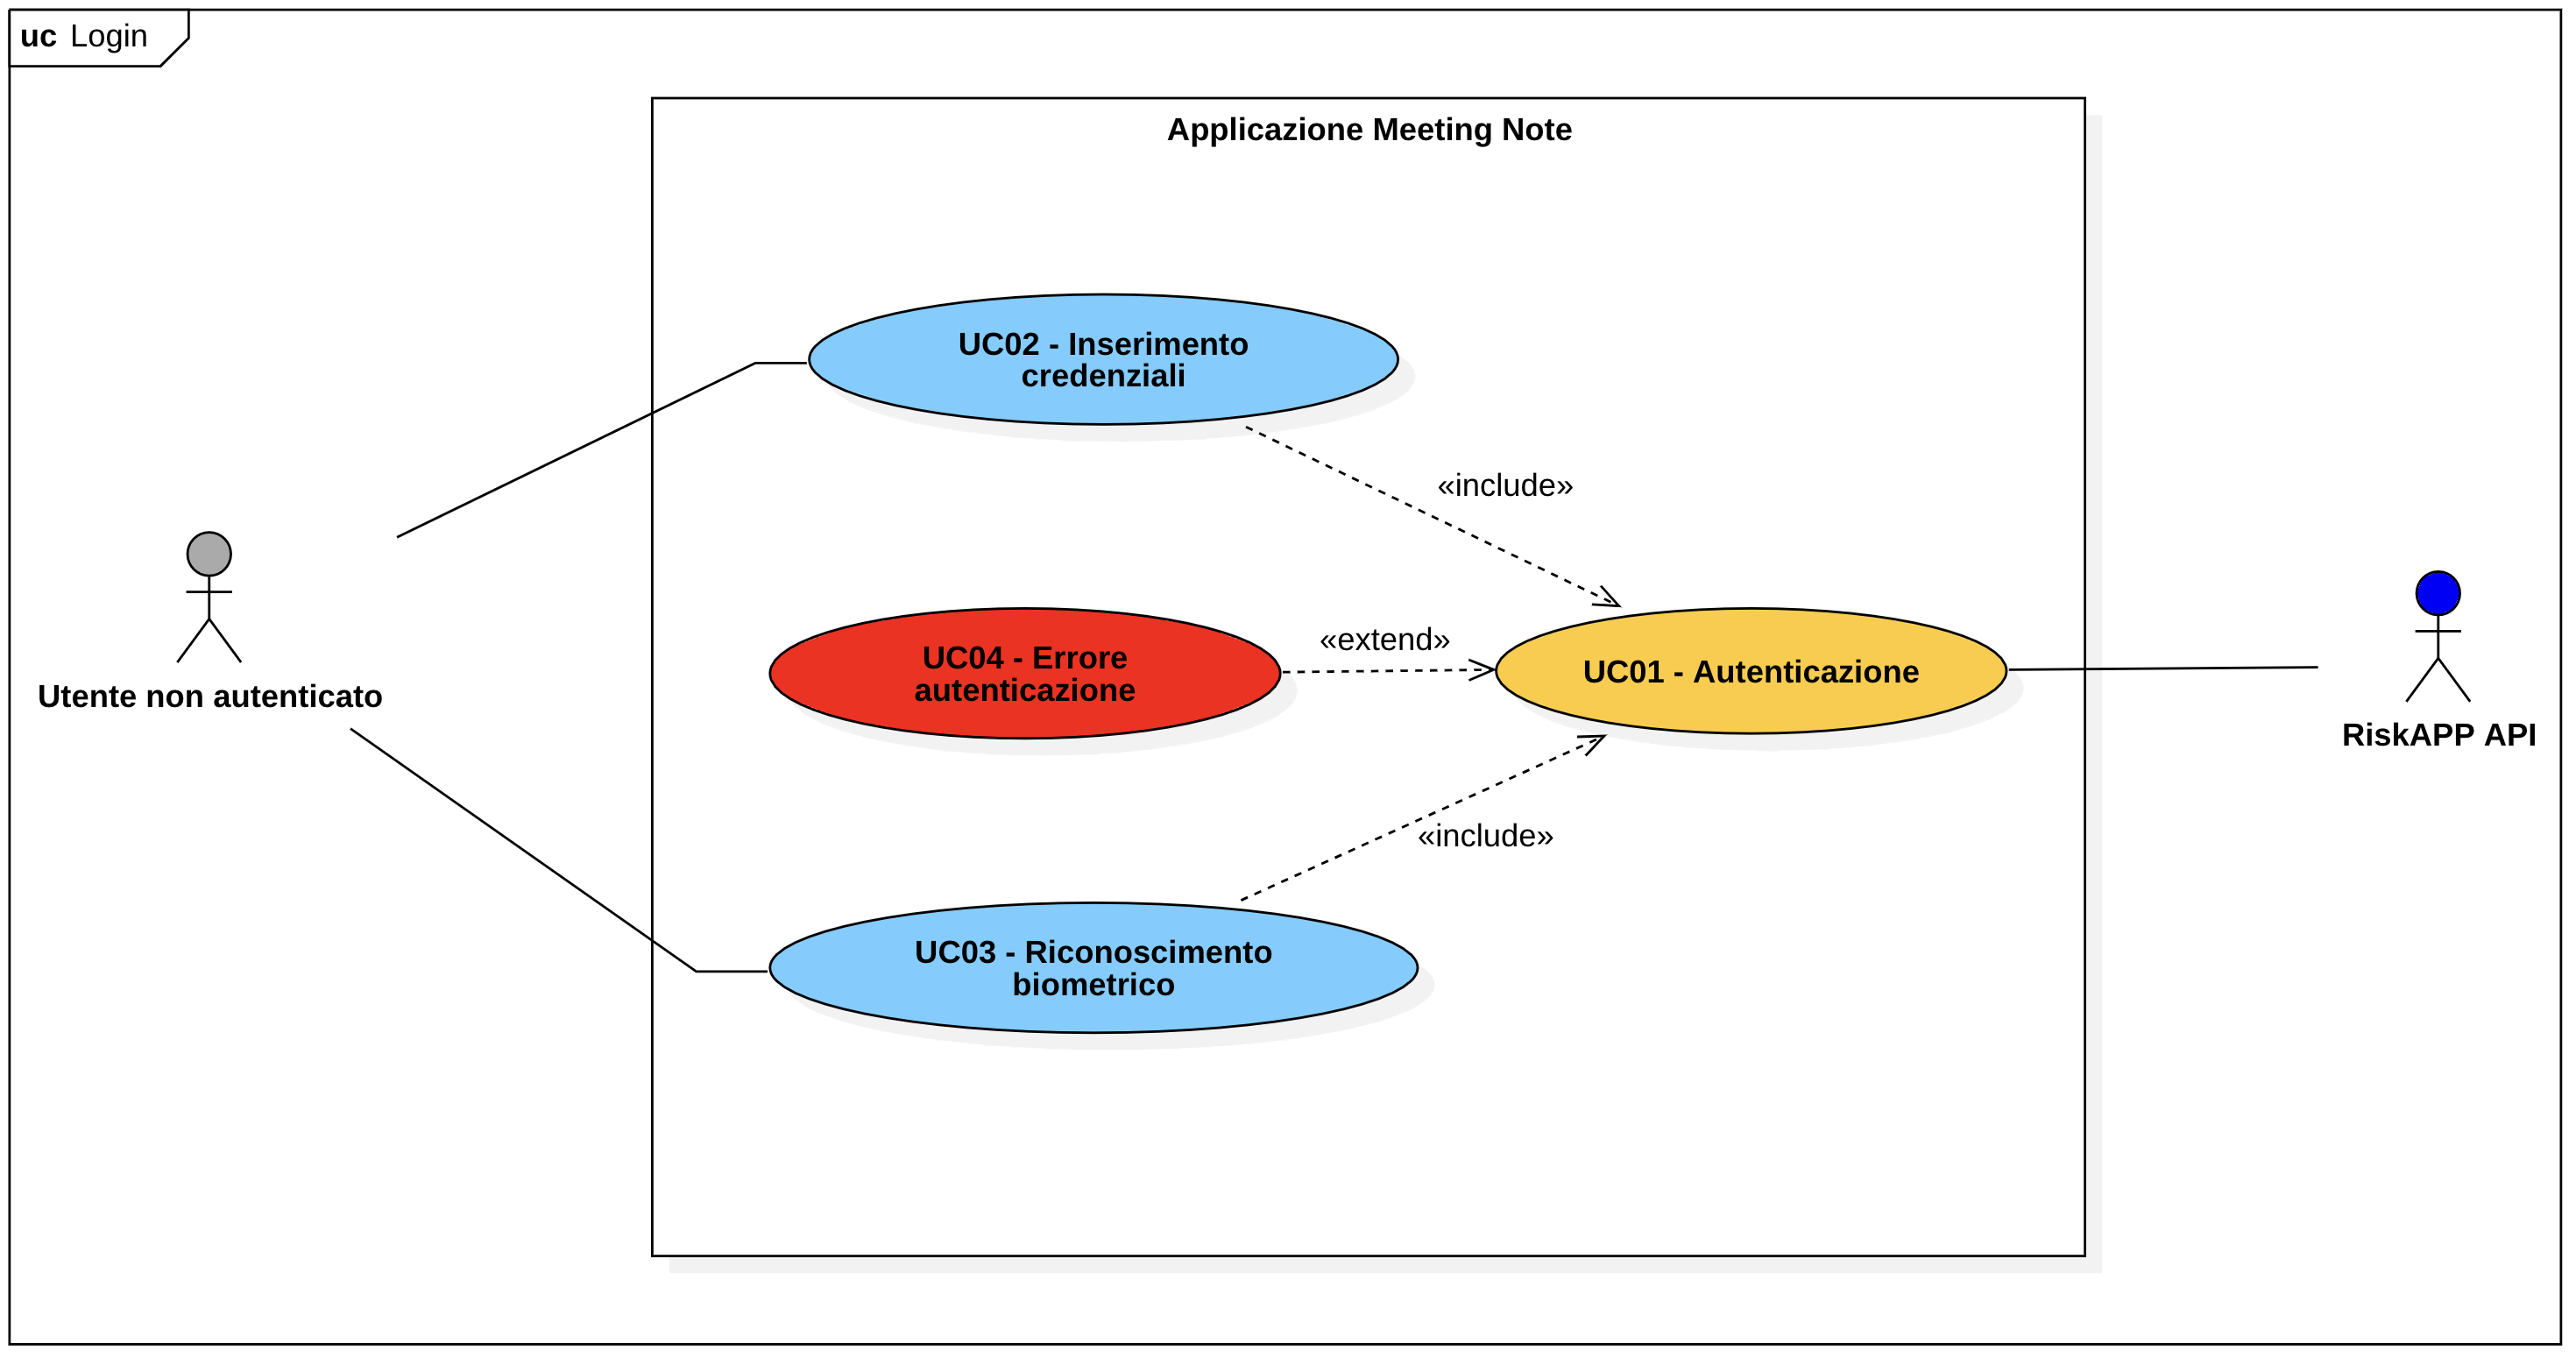
\includegraphics[width=1.0\columnwidth]{usecase/1-uc} 
    \caption{Use Case - Autenticazione}
    \label{fig:uc-login}
\end{figure}

\begin{usecase}{01}{Autenticazione}
    \usecasemainactors{Utente non autenticato}
    \usecasesecondaryactors{\emph{RiskAPP API}}
    \usecasepre{L'utente non è ancora autenticato nel sistema}
    \usecasedesc{L'utente effettua l'autenticazione al sistema, scegliendo se farlo, inserendo manualmente le credenziali, oppure tramite \gls{riconoscimentobiometrico}\glsoccur.}
    \usecasepost{L'utente è autenticato nel sistema}
    \usecasealt{Se l'autenticazione fallisce, si verifica \hyperref[UC04]{UC04}}
    \usecaseimg{\ref{fig:uc-login}}
    \label{UC01}
\end{usecase}

\begin{usecase}{02}{Inserimento credenziali}
    \usecasemainactors{Utente non autenticato}
    \usecasepre{L'utente non è ancora autenticato nel sistema}
    \usecasedesc{L'utente inserisce manualmente le proprie credenziali per effettuare l'autenticazione al sistema.}
    \usecasepost{L'utente è autenticato nel sistema}
    \usecaseimg{\ref{fig:uc-login}}
    \label{UC02}
\end{usecase}

\newpage

\begin{usecase}{03}{Riconoscimento biometrico}
    \usecasemainactors{Utente non autenticato}
    \usecasepre{L'utente non è ancora autenticato nel sistema}
    \usecasedesc{L'utente utilizza il \gls{riconoscimentobiometrico}\glsoccur per effettuare l'autenticazione al sistema.}
    \usecasepost{L'utente è autenticato nel sistema}
    \usecaseimg{\ref{fig:uc-login}}
    \label{UC03}
\end{usecase}

\begin{usecase}{04}{Errore autenticazione}
    \usecasemainactors{Utente non autenticato}
    \usecasesecondaryactors{\emph{RiskAPP API}}
    \usecasepre{L'utente non è ancora autenticato nel sistema}
    \usecasedesc{L'autenticazione fallisce e l'utente viene informato dell'errore; le motivazioni possono essere le seguenti:
        \begin{itemize}
            \item le credenziali inserite non sono corrette;
            \item il sistema non è raggiungibile o connessione ad internet assente;
            \item il \gls{riconoscimentobiometrico}\glsoccur è fallito.
        \end{itemize}}
    \usecasepost{L'utente non è autenticato nel sistema}
    \usecaseimg{\ref{fig:uc-login}}
    \label{UC04}
\end{usecase}

\begin{figure}[!h] 
    \centering 
    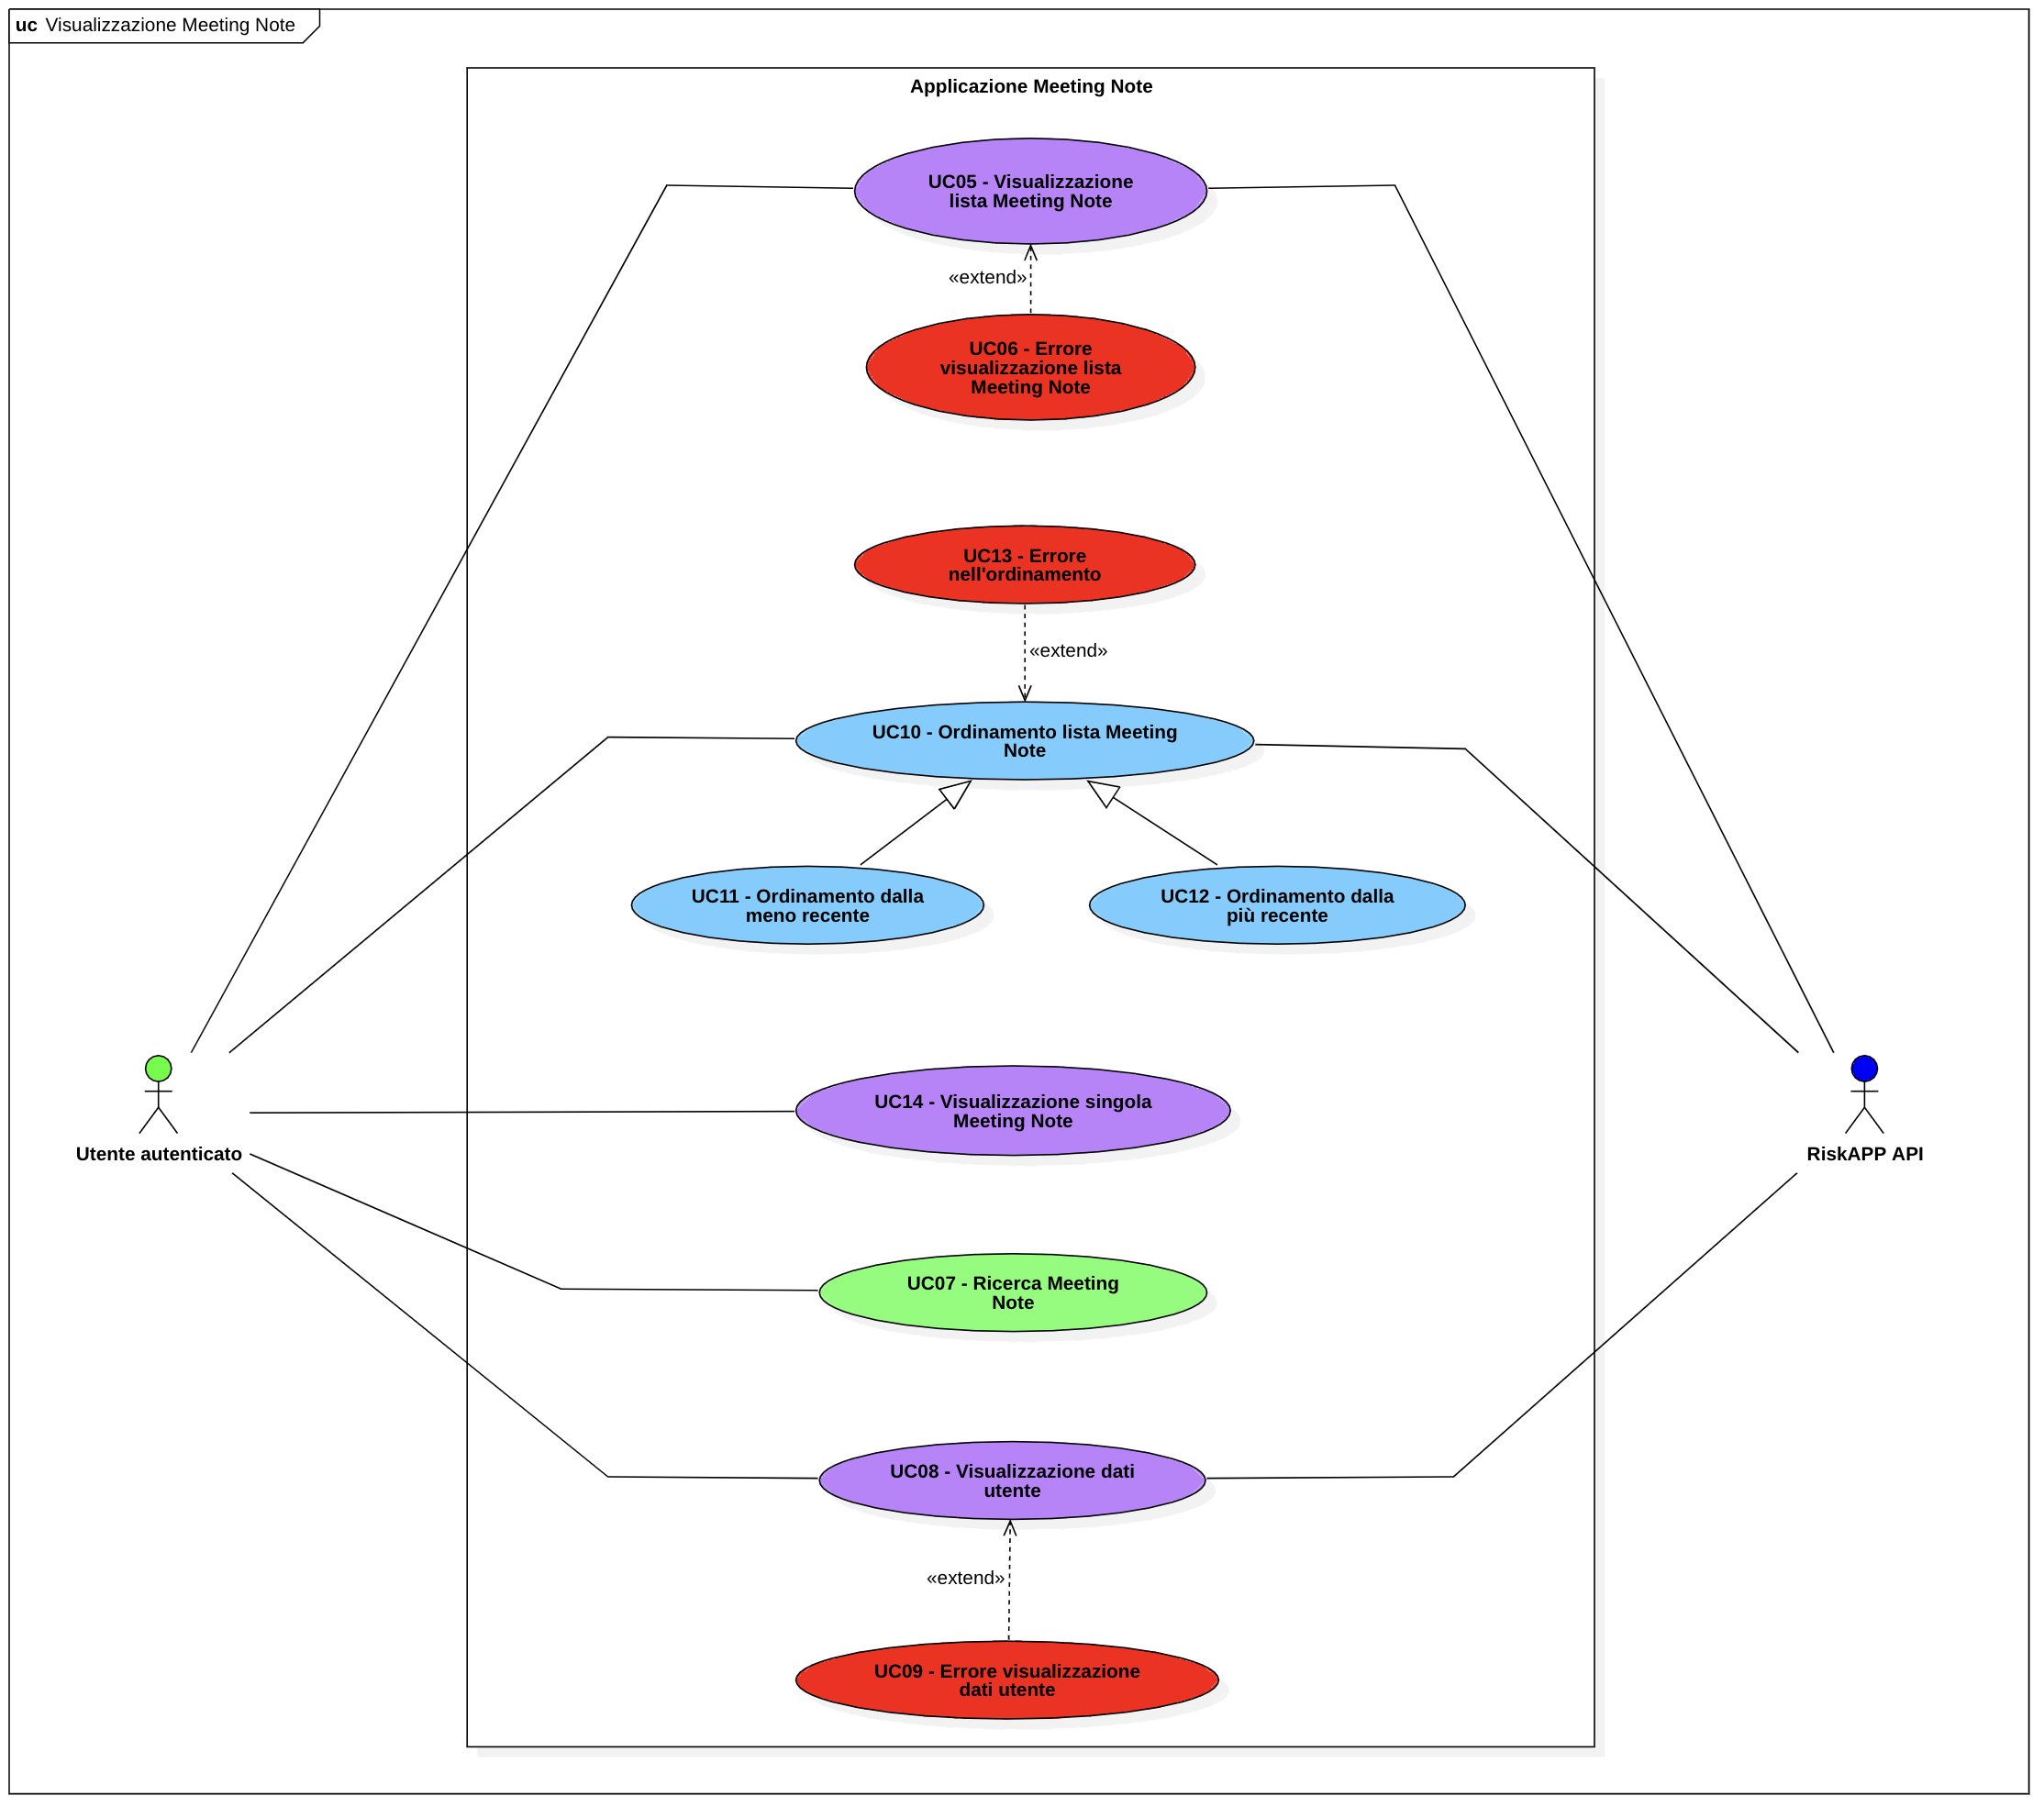
\includegraphics[width=1.0\columnwidth]{usecase/2-uc} 
    \caption{Use Case - Visualizzazione Meeting Note}
    \label{fig:uc-meetingnote}
\end{figure}

\begin{usecase}{05}{Visualizzazione lista Meeting Note}
    \usecasemainactors{Utente autenticato}
    \usecasesecondaryactors{\emph{RiskAPP API}}
    \usecasepre{L'utente è autenticato nel sistema}
    \usecasedesc{L'utente vuole visualizzare la lista di tutte le \gls{meetingnote}\glsoccur associate.}
    \usecasepost{È visualizzabile la lista delle \gls{meetingnote}\glsoccur}
    \usecasealt{Se la visualizzazione fallisce, si verifica \hyperref[UC06]{UC06}}
    \usecaseimg{\ref{fig:uc-meetingnote}}
    \label{UC05}
\end{usecase}

\begin{figure}[!h] 
    \centering 
    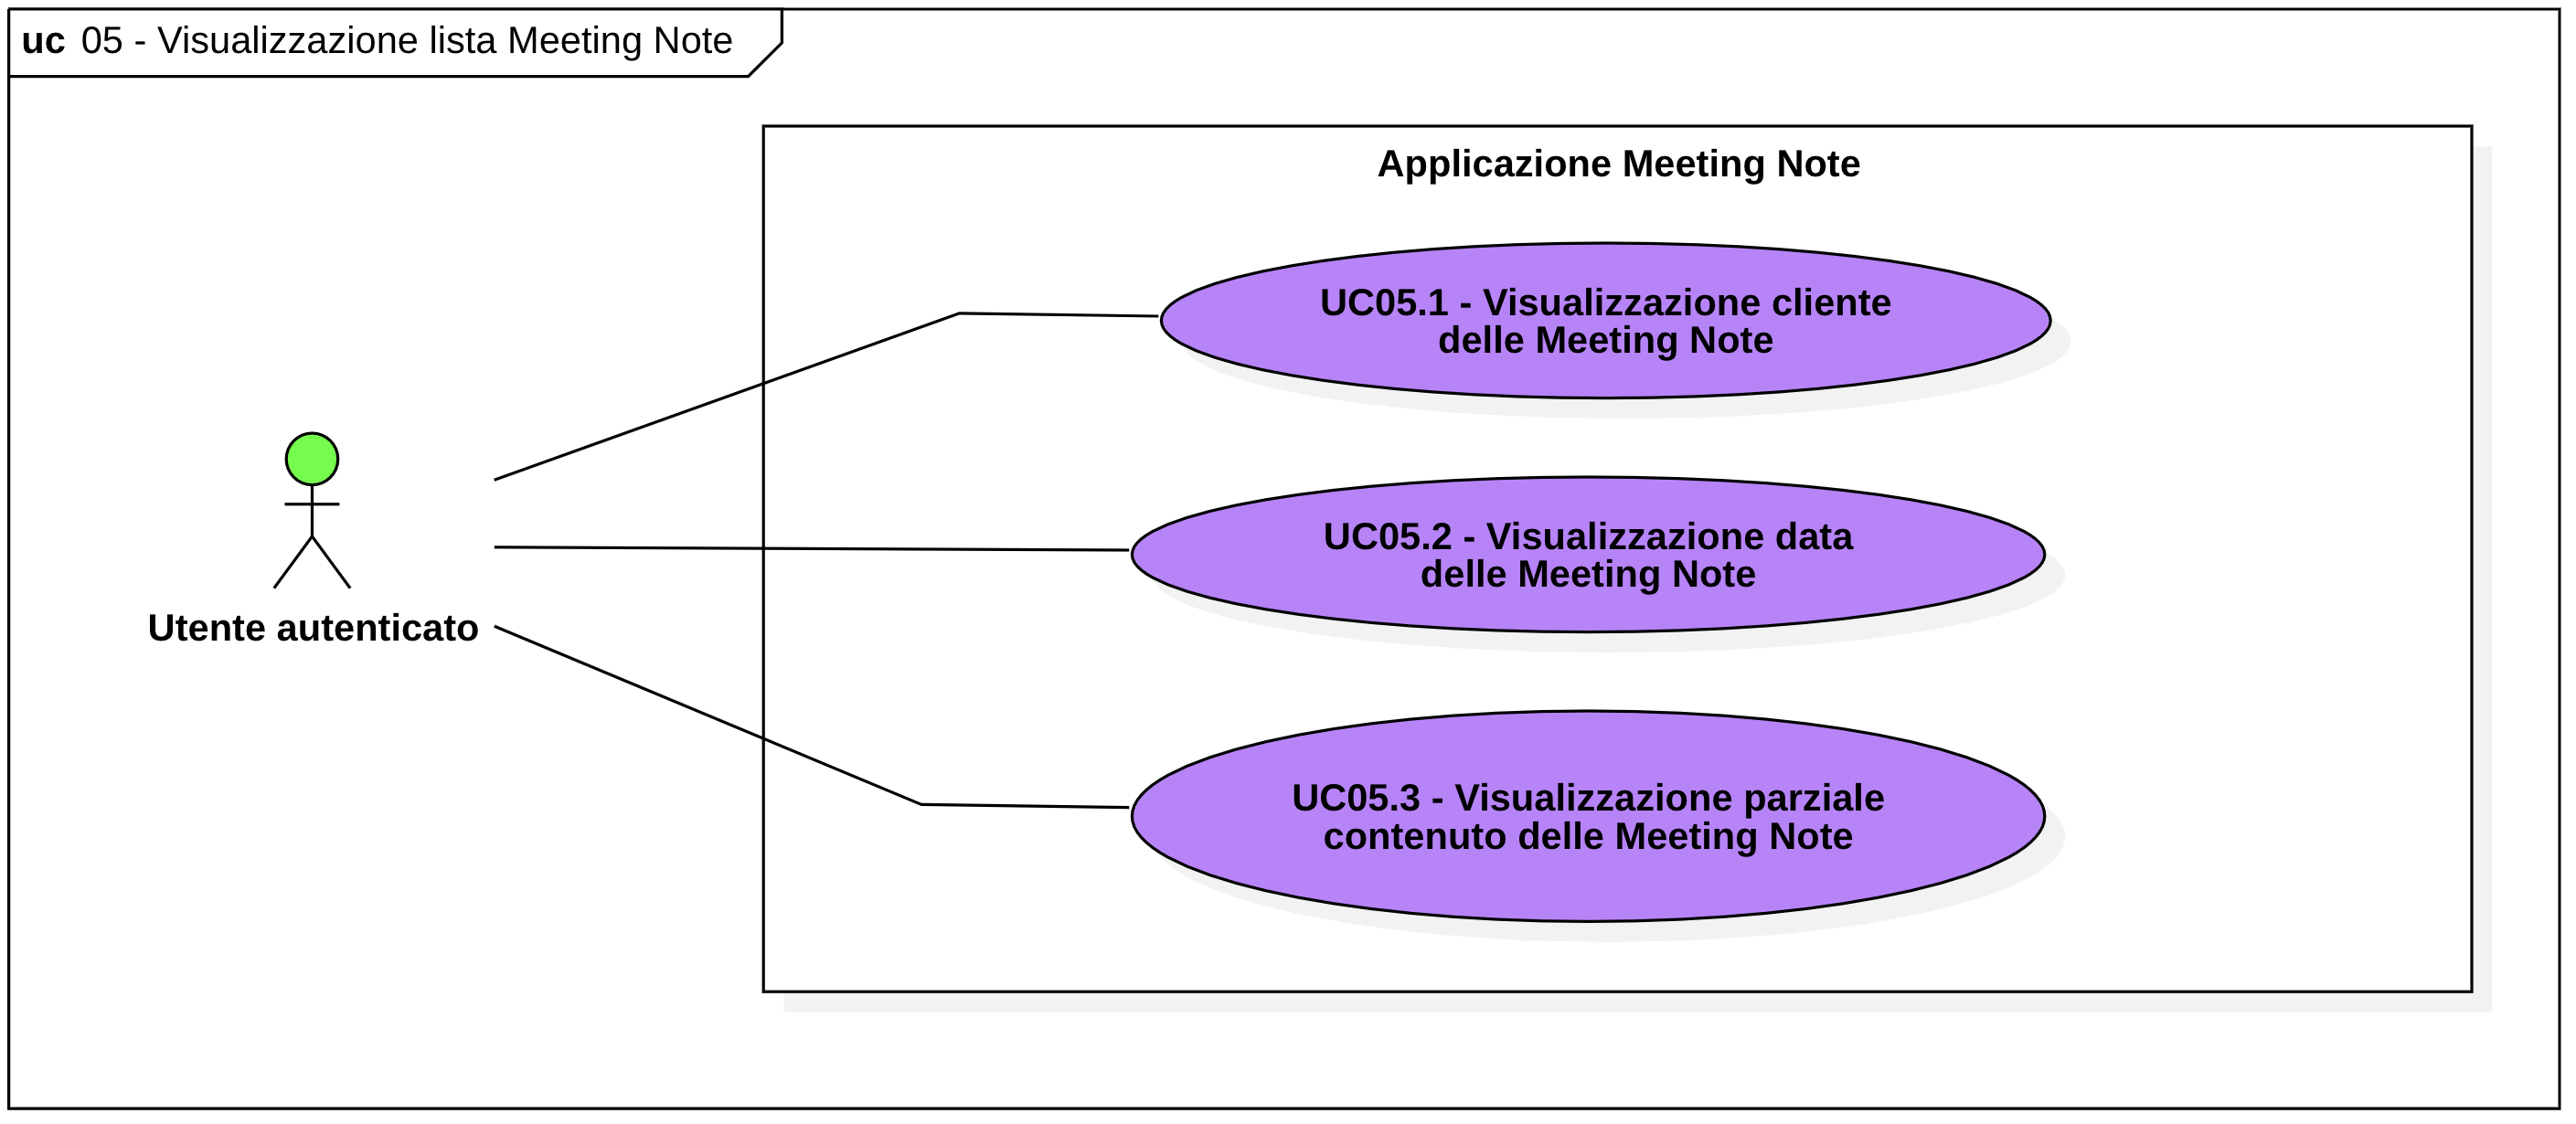
\includegraphics[width=1.0\columnwidth]{usecase/3-uc} 
    \caption{Use Case - Visualizzazione lista Meeting Note}
    \label{fig:uc-meetingnote-list-details}
\end{figure}

\begin{usecase}{05.1}{Visualizzazione cliente delle Meeting Note}
    \usecasemainactors{Utente autenticato}
    \usecasepre{L'utente visualizza la lista delle \gls{meetingnote}\glsoccur}
    \usecasedesc{L'utente vuole visualizzare gli identificativi dei \glspl{cliente}\glsoccur associati alle \gls{meetingnote}\glsoccur.}
    \usecasepost{Sono visualizzabili i \glspl{cliente}\glsoccur associati alle \gls{meetingnote}\glsoccur}
    \usecaseimg{\ref{fig:uc-meetingnote-list-details}}
    \label{UC05.1}
\end{usecase}

\clearpage

\begin{usecase}{05.2}{Visualizzazione data della Meeting Note}
    \usecasemainactors{Utente autenticato}
    \usecasepre{L'utente visualizza la lista delle \gls{meetingnote}\glsoccur}
    \usecasedesc{L'utente vuole visualizzare le date degli incontri associati alle \gls{meetingnote}\glsoccur.}
    \usecasepost{Sono visualizzabili le date degli incontri associati alle \gls{meetingnote}\glsoccur}
    \usecaseimg{\ref{fig:uc-meetingnote-list-details}}
    \label{UC05.2}
\end{usecase}

\begin{usecase}{05.3}{Visualizzazione parziale contenuto delle Meeting Note}
    \usecasemainactors{Utente autenticato}
    \usecasepre{L'utente visualizza la lista delle \gls{meetingnote}\glsoccur}
    \usecasedesc{L'utente vuole visualizzare parzialmente i contenuti delle \gls{meetingnote}\glsoccur.}
    \usecasepost{Sono visualizzabili parzialmente i contenuti delle \gls{meetingnote}\glsoccur}
    \usecaseimg{\ref{fig:uc-meetingnote-list-details}}
    \label{UC05.3}
\end{usecase}

\begin{usecase}{06}{Errore visualizzazione lista Meeting Note}
    \usecasemainactors{Utente autenticato}
    \usecasesecondaryactors{\emph{RiskAPP API}}
    \usecasepre{L'utente è autenticato nel sistema}
    \usecasedesc{La visualizzazione della lista delle \gls{meetingnote}\glsoccur fallisce e l'utente viene informato dell'errore; le motivazioni possono essere le seguenti:
        \begin{itemize}
            \item la lista è vuota;
            \item il sistema non è raggiungibile;
            \item token di autenticazione scaduto;
            \item connessione ad internet assente.
        \end{itemize}}
    \usecasepost{Non è visualizzabile la lista delle \gls{meetingnote}\glsoccur}
    \usecaseimg{\ref{fig:uc-meetingnote}}
    \label{UC06}
\end{usecase}

\begin{usecase}{07}{Ricerca Meeting Note}
    \usecasemainactors{Utente autenticato}
    \usecasepre{L'utente visualizza la lista delle \gls{meetingnote}\glsoccur a lui associate}
    \usecasedesc{L'utente effettua una ricerca all'interno della lista delle \gls{meetingnote}\glsoccur.}
    \usecasepost{Lista delle \gls{meetingnote}\glsoccur è filtrata}
    \usecaseimg{\ref{fig:uc-meetingnote}}
    \label{UC07}
\end{usecase}

\newpage

\begin{figure}[!h] 
    \centering 
    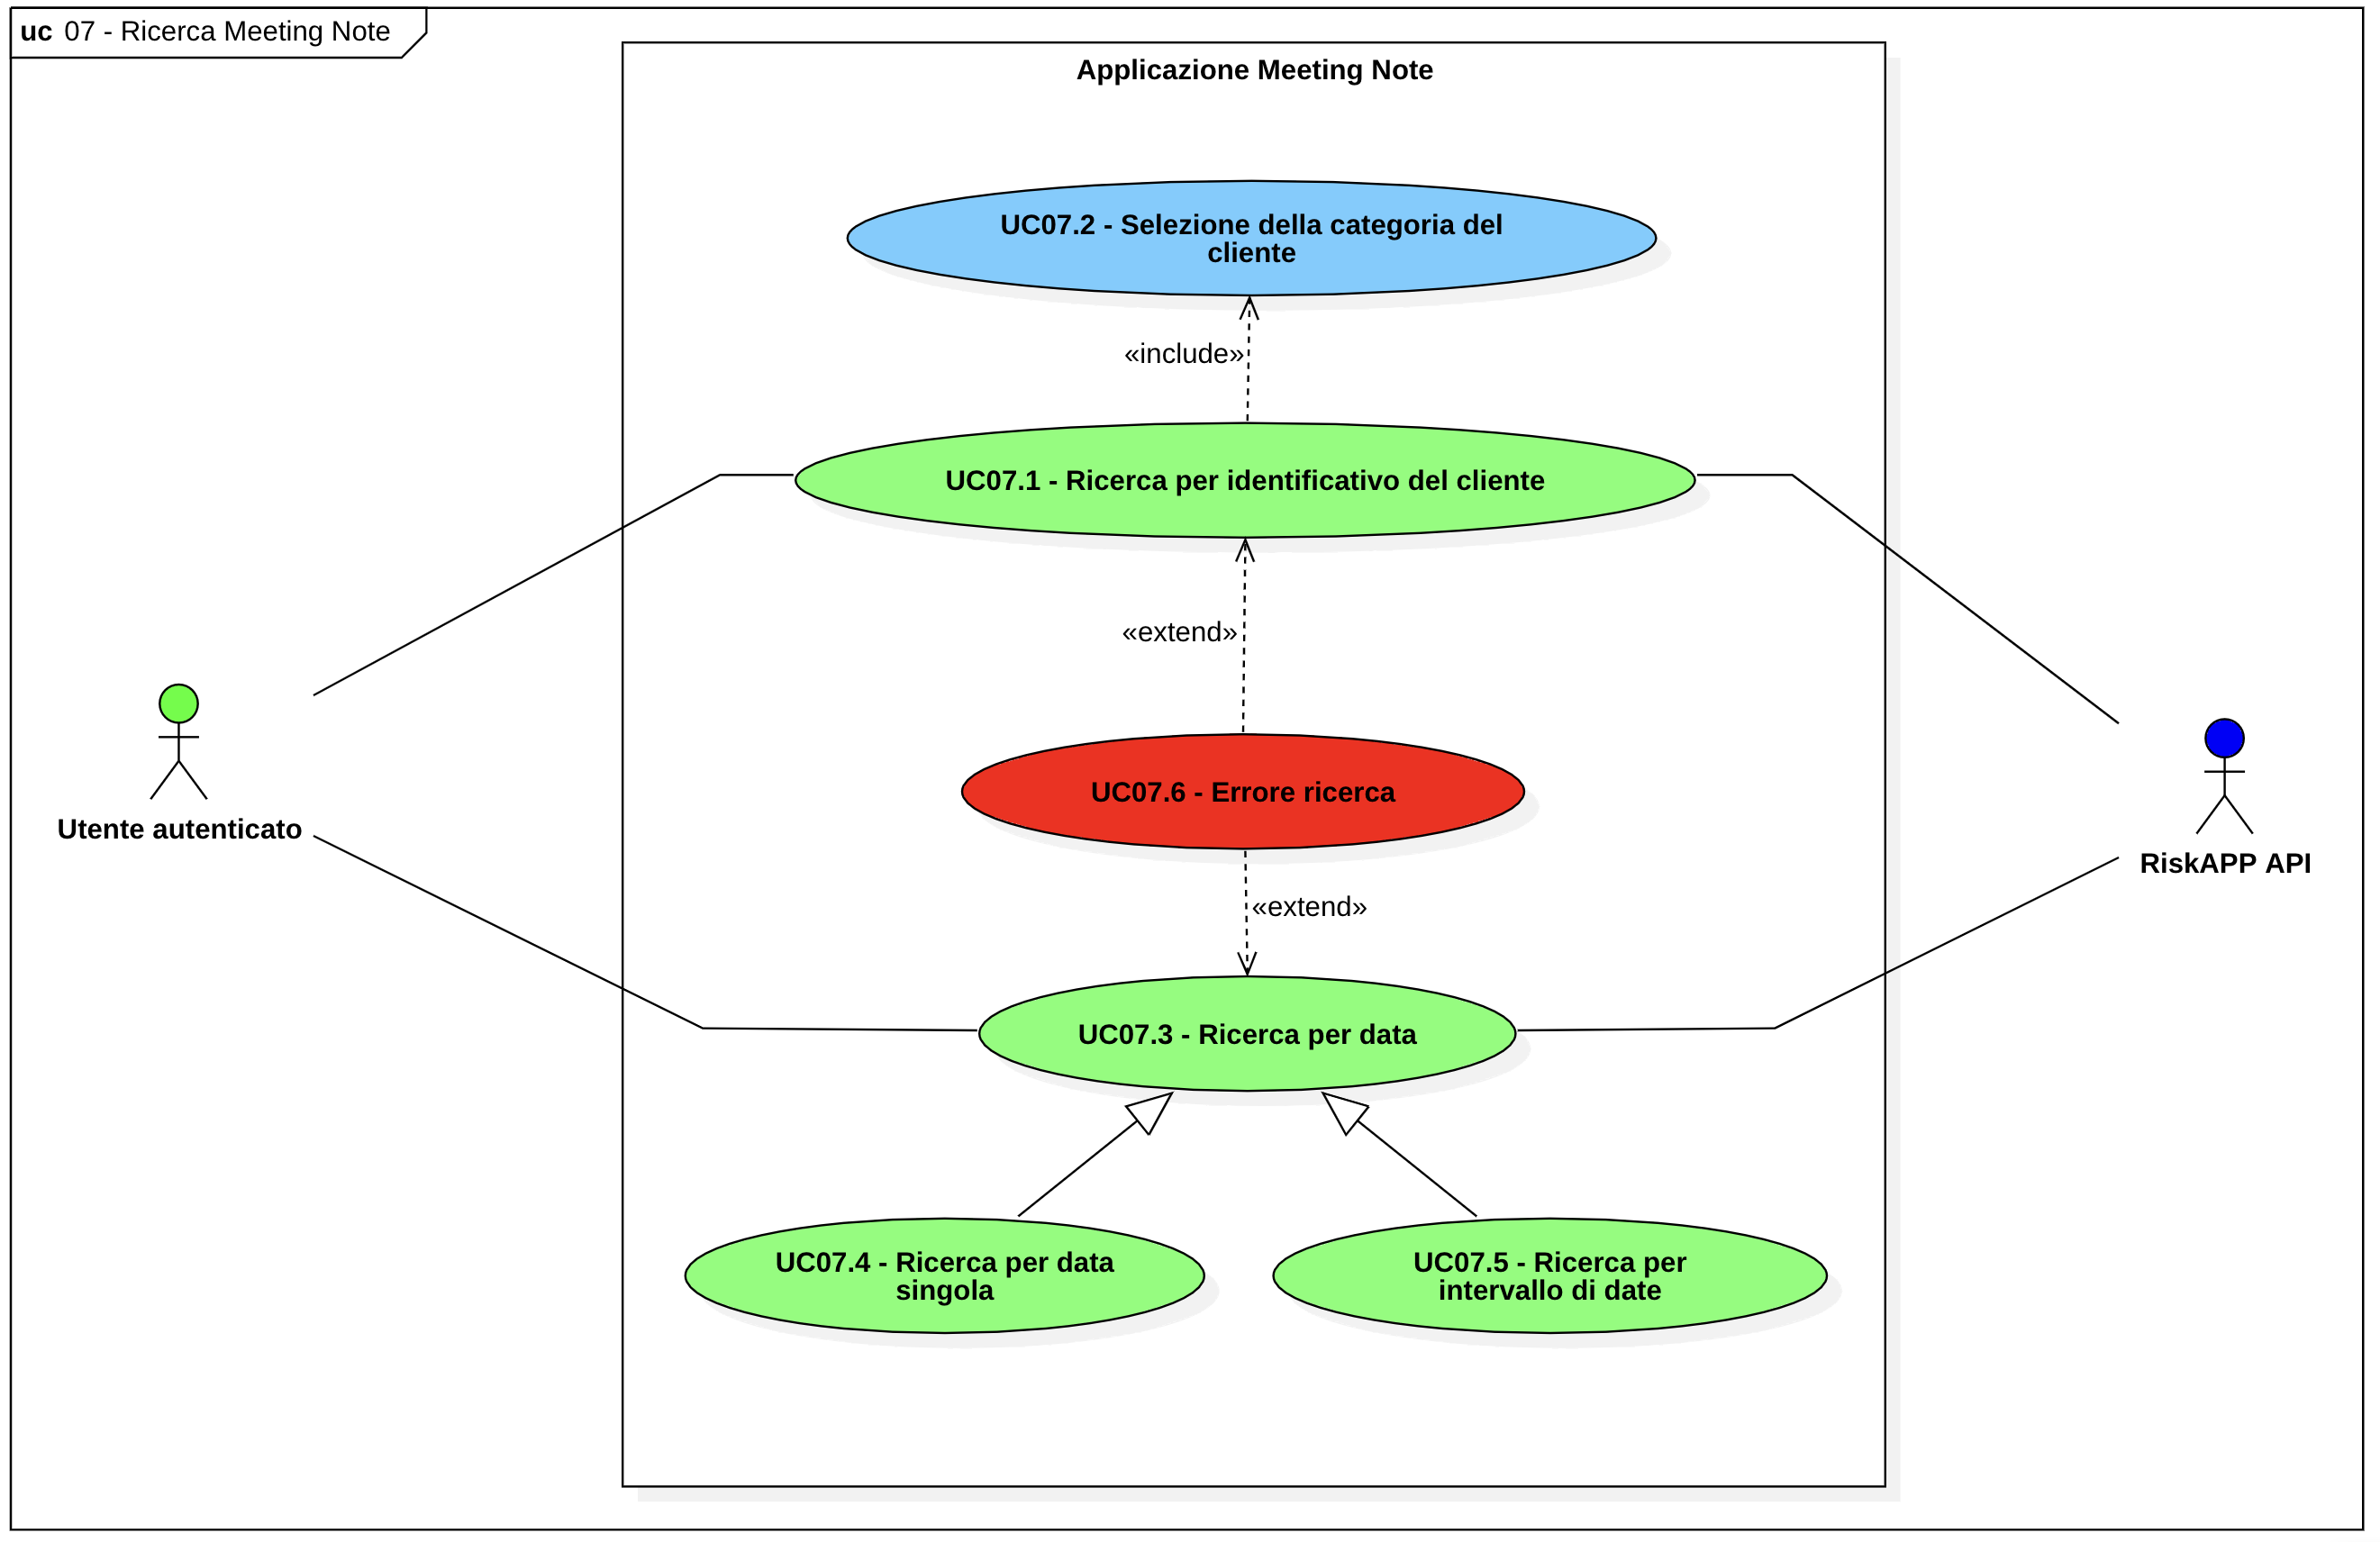
\includegraphics[width=1.0\columnwidth]{usecase/4-uc} 
    \caption{Use Case - Ricerca Meeting Note}
    \label{fig:uc-meetingnote-search}
\end{figure}

\begin{usecase}{07.1}{Ricerca per identificativo del cliente}
    \usecasemainactors{Utente autenticato}
    \usecasesecondaryactors{\emph{RiskAPP API}}
    \usecasepre{L'utente ha selezionato la categoria del \gls{cliente}\glsoccur}
    \usecasedesc{L'utente effettua una ricerca per identificativo del \gls{cliente}\glsoccur all'interno della lista delle \gls{meetingnote}\glsoccur.}
    \usecasepost{Lista delle \gls{meetingnote}\glsoccur è filtrata per identificativo del \gls{cliente}\glsoccur}
    \usecasealt{Se la ricerca fallisce, si verifica \hyperref[UC07.6]{UC07.6}}
    \usecaseimg{\ref{fig:uc-meetingnote-search}}
    \label{UC07.1}
\end{usecase}

\begin{usecase}{07.2}{Selezione della categoria del cliente}
    \usecasemainactors{Utente autenticato}
    \usecasepre{L'utente visualizza la lista delle \gls{meetingnote}\glsoccur a lui associate}
    \usecasedesc{L'utente seleziona la categoria del \gls{cliente}\glsoccur per effettuare la ricerca per identificativo all'interno della lista delle \gls{meetingnote}\glsoccur.}
    \usecasepost{La categoria del \gls{cliente}\glsoccur è selezionata}
    \usecaseimg{\ref{fig:uc-meetingnote-search}}
    \label{UC07.2}
\end{usecase}

\begin{usecase}{07.3}{Ricerca per data}
    \usecasemainactors{Utente autenticato}
    \usecasesecondaryactors{\emph{RiskAPP API}}
    \usecasepre{L'utente visualizza la lista delle \gls{meetingnote}\glsoccur a lui associate}
    \usecasedesc{L'utente effettua una ricerca per data all'interno della lista delle \gls{meetingnote}\glsoccur.}
    \usecasepost{Lista delle \gls{meetingnote}\glsoccur è filtrata per data}
    \usecasealt{Se la ricerca fallisce, si verifica \hyperref[UC07.6]{UC07.6}}
    \usecaseimg{\ref{fig:uc-meetingnote-search}}
    \label{UC07.3}
\end{usecase}

\begin{usecase}{07.4}{Ricerca per data singola}
    \usecasemainactors{Utente autenticato}
    \usecasepre{L'utente visualizza la lista delle \gls{meetingnote}\glsoccur a lui associate}
    \usecasedesc{L'utente effettua una ricerca per data singola all'interno della lista delle \gls{meetingnote}\glsoccur.}
    \usecasepost{Lista delle \gls{meetingnote}\glsoccur è filtrata per data singola}
    \usecaseimg{\ref{fig:uc-meetingnote-search}}
    \label{UC07.4}
\end{usecase}

\begin{usecase}{07.5}{Ricerca per intervallo di date}
    \usecasemainactors{Utente autenticato}
    \usecasepre{L'utente visualizza la lista delle \gls{meetingnote}\glsoccur a lui associate}
    \usecasedesc{L'utente effettua una ricerca per intervallo di date all'interno della lista delle \gls{meetingnote}\glsoccur.}
    \usecasepost{Lista delle \gls{meetingnote}\glsoccur è filtrata per intervallo di date}
    \usecaseimg{\ref{fig:uc-meetingnote-search}}
    \label{UC07.5}
\end{usecase}

\begin{usecase}{07.6}{Errore ricerca}
    \usecasemainactors{Utente autenticato}
    \usecasesecondaryactors{\emph{RiskAPP API}}
    \usecasepre{L'utente ha effettuato una ricerca all'interno della lista delle \gls{meetingnote}\glsoccur}
    \usecasedesc{La ricerca fallisce e l'utente viene informato dell'errore; le motivazioni possono essere le seguenti:
        \begin{itemize}
            \item la lista risultante è vuota;
            \item il sistema non è raggiungibile;
            \item token di autenticazione scaduto;
            \item connessione ad internet assente.
        \end{itemize}}
    \usecasepost{Lista delle \gls{meetingnote}\glsoccur non è filtrata}
    \usecaseimg{\ref{fig:uc-meetingnote-search}}
    \label{UC07.6}
\end{usecase}

\begin{usecase}{08}{Visualizzazione dati utente}
    \usecasemainactors{Utente autenticato}
    \usecasesecondaryactors{\emph{RiskAPP API}}
    \usecasepre{L'utente è autenticato nel sistema}
    \usecasedesc{L'utente vuole visualizzare i propri dati personali.}
    \usecasepost{Sono visualizzabili i dati personali dell'utente}
    \usecasealt{Se la visualizzazione fallisce, si verifica \hyperref[UC09]{UC09}} 
    \usecaseimg{\ref{fig:uc-meetingnote}}
    \label{UC08}
\end{usecase}

\begin{figure}[!h] 
    \centering 
    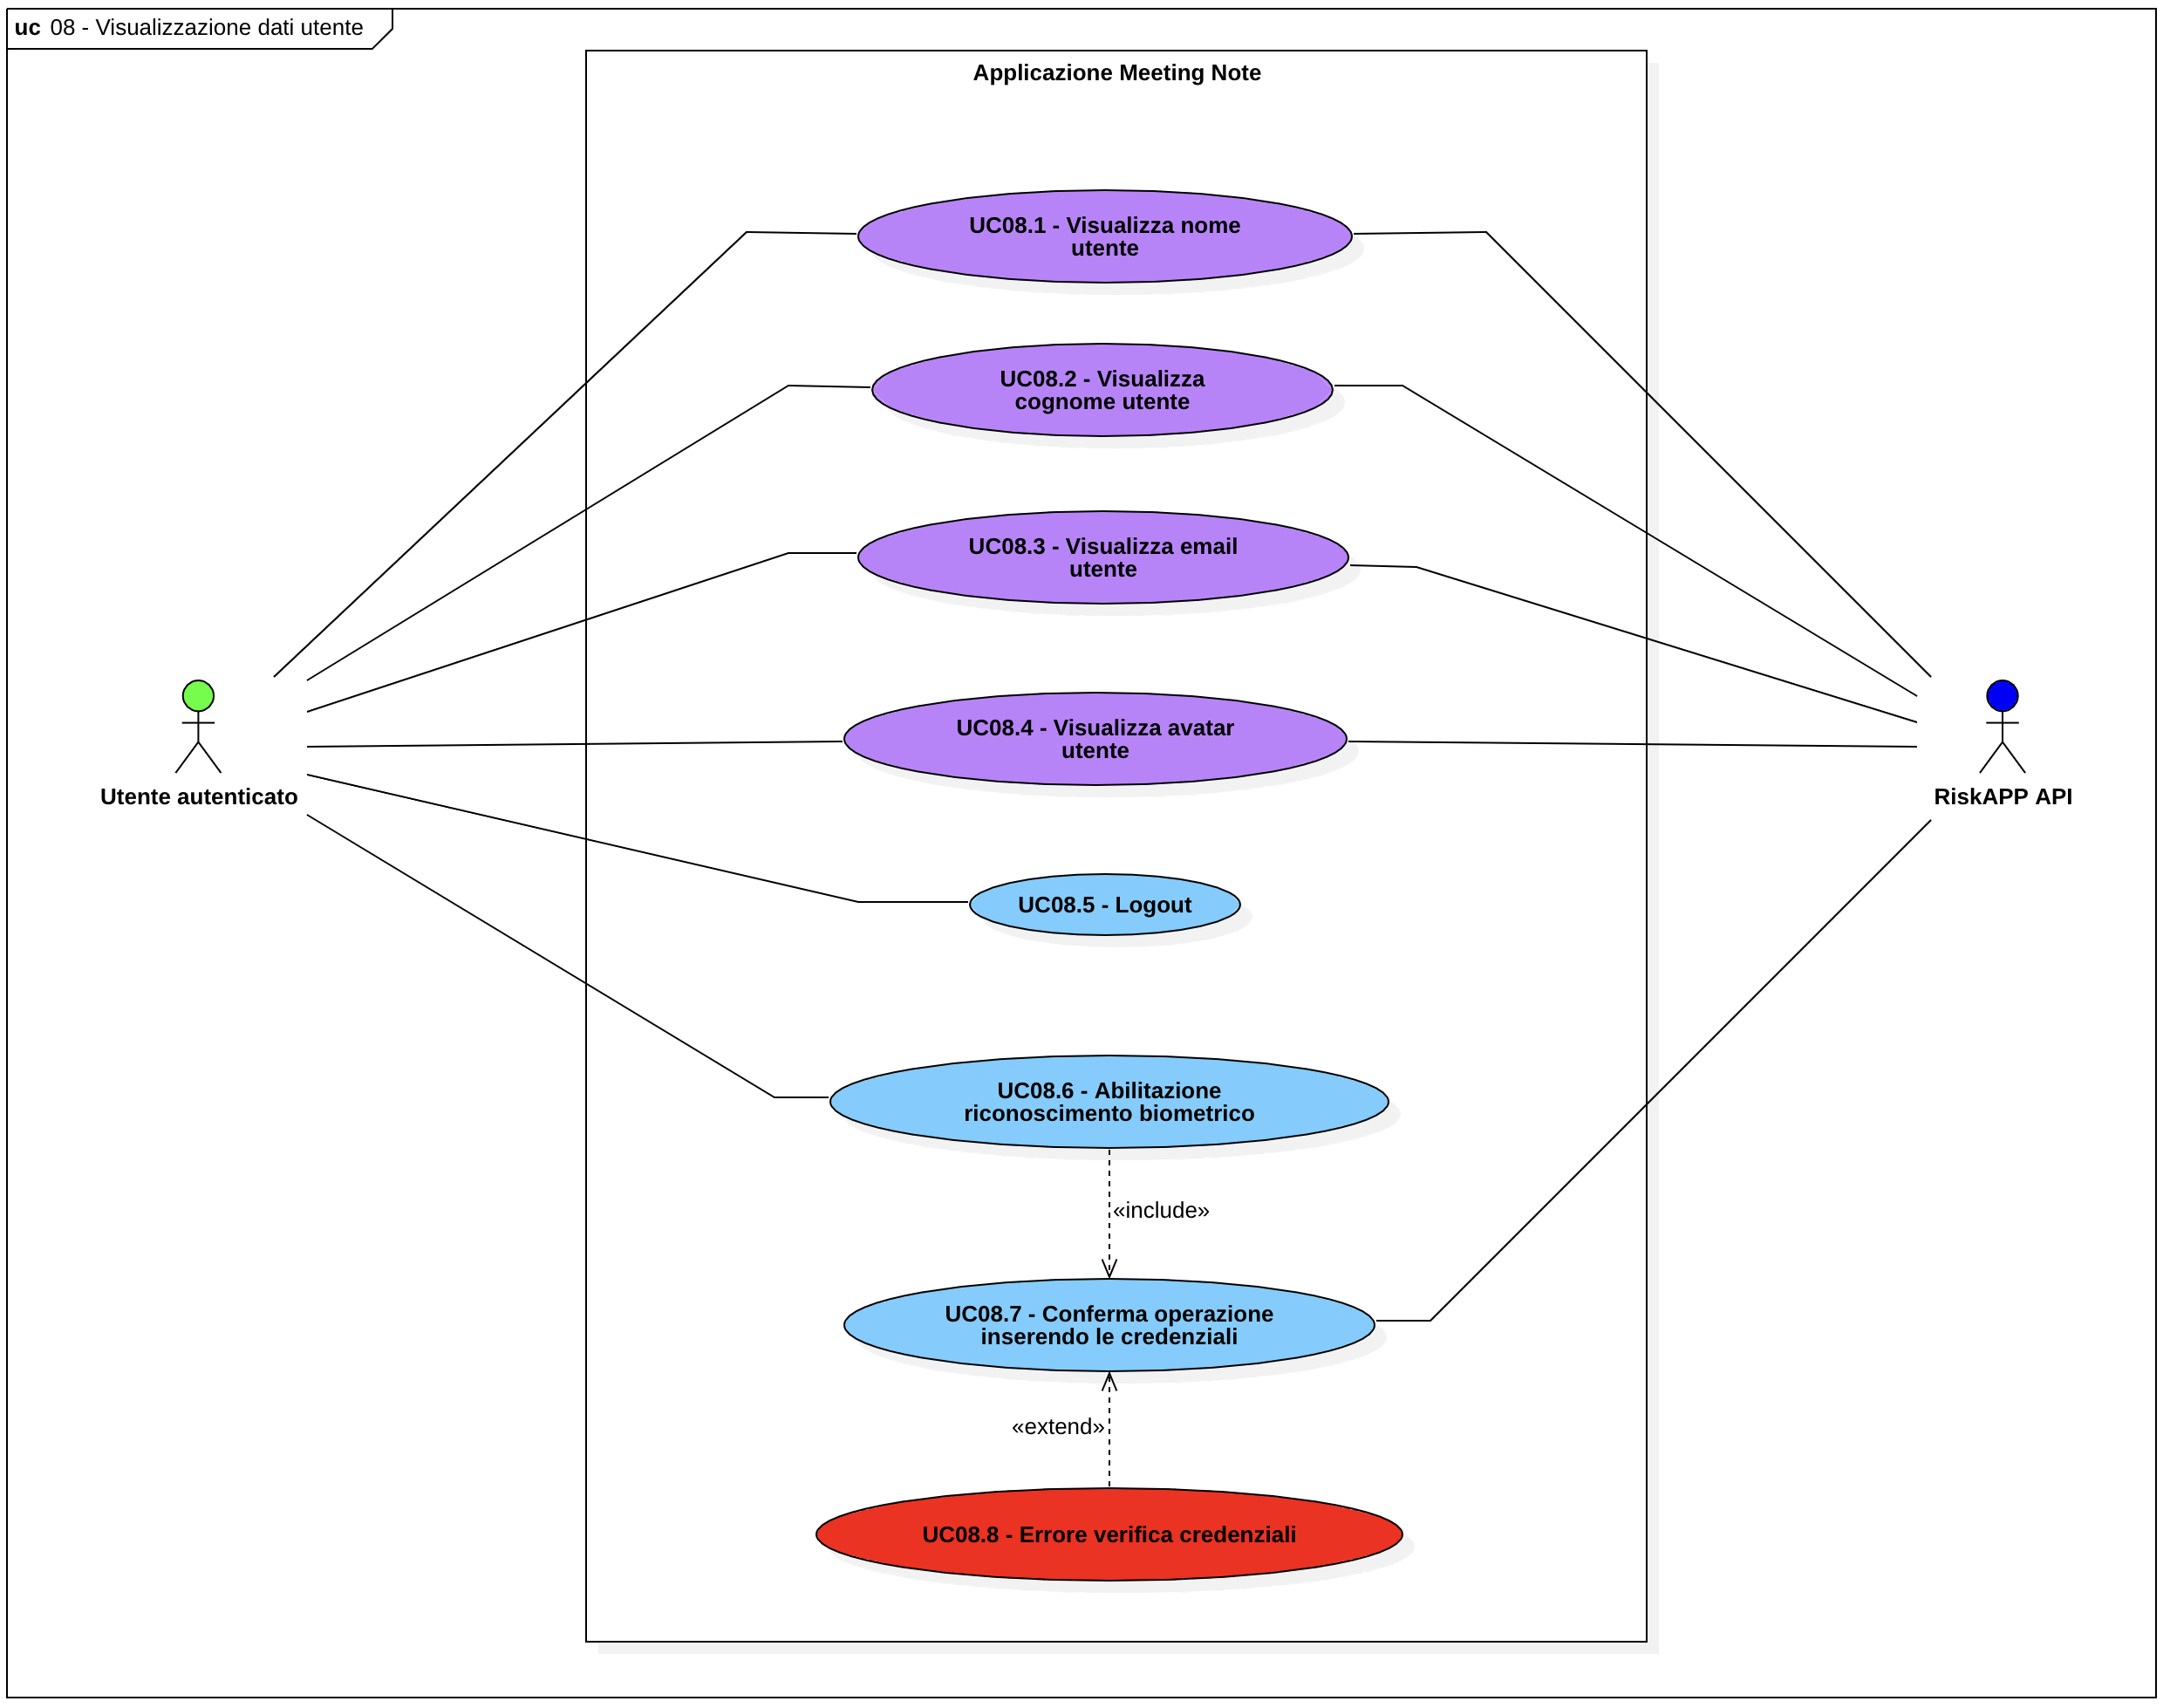
\includegraphics[width=1.0\columnwidth]{usecase/5-uc} 
    \caption{Use Case - Visualizzazione dati utente}
    \label{fig:uc-user}
\end{figure}

\begin{usecase}{08.1}{Visualizzazione nome utente}
    \usecasemainactors{Utente autenticato}
    \usecasesecondaryactors{\emph{RiskAPP API}}
    \usecasepre{L'utente visualizza i propri dati personali}
    \usecasedesc{L'utente vuole visualizzare il proprio nome.}
    \usecasepost{È visualizzabile il nome dell'utente}
    \usecaseimg{\ref{fig:uc-user}}
    \label{UC08.1}
\end{usecase}

\begin{usecase}{08.2}{Visualizzazione cognome utente}
    \usecasemainactors{Utente autenticato}
    \usecasesecondaryactors{\emph{RiskAPP API}}
    \usecasepre{L'utente visualizza i propri dati personali}
    \usecasedesc{L'utente vuole visualizzare il proprio cognome.}
    \usecasepost{È visualizzabile il cognome dell'utente}
    \usecaseimg{\ref{fig:uc-user}}
    \label{UC08.2}
\end{usecase}

\begin{usecase}{08.3}{Visualizzazione email utente}
    \usecasemainactors{Utente autenticato}
    \usecasesecondaryactors{\emph{RiskAPP API}}
    \usecasepre{L'utente visualizza i propri dati personali}
    \usecasedesc{L'utente vuole visualizzare la propria email.}
    \usecasepost{È visualizzabile la email dell'utente}
    \usecaseimg{\ref{fig:uc-user}}
    \label{UC08.3}
\end{usecase}

\begin{usecase}{08.4}{Visualizzazione avatar utente}
    \usecasemainactors{Utente autenticato}
    \usecasesecondaryactors{\emph{RiskAPP API}}
    \usecasepre{L'utente visualizza i propri dati personali}
    \usecasedesc{L'utente vuole visualizzare il proprio avatar.}
    \usecasepost{È visualizzabile l'avatar dell'utente}
    \usecaseimg{\ref{fig:uc-user}}
    \label{UC08.4}
\end{usecase}

\begin{usecase}{08.5}{Logout}
    \usecasemainactors{Utente autenticato}
    \usecasepre{L'utente visualizza i propri dati personali}
    \usecasedesc{L'utente vuole effetuare il logout.}
    \usecasepost{L'utente non è più autenticato al sistema}
    \usecaseimg{\ref{fig:uc-user}}
    \label{UC08.5}
\end{usecase}

\begin{usecase}{08.6}{Abilitazione riconoscimento biometrico}
    \usecasemainactors{Utente autenticato}
    \usecasesecondaryactors{\emph{RiskAPP API}}
    \usecasepre{L'utente visualizza i propri dati personali}
    \usecasedesc{L'utente vuole abilitare il \gls{riconoscimentobiometrico}\glsoccur, deve inserire le proprie credenziali per la conferma.}
    \usecasepost{Riconoscimento biometrico abilitato}
    \usecaseimg{\ref{fig:uc-user}}
    \label{UC08.6}
\end{usecase}

\begin{usecase}{08.7}{Conferma operazione inserendo le credenziali}
    \usecasemainactors{Utente autenticato}
    \usecasesecondaryactors{\emph{RiskAPP API}}
    \usecasepre{L'utente visualizza i propri dati personali}
    \usecasedesc{L'utente inserisce le proprie credenziali per abilitare il \gls{riconoscimentobiometrico}\glsoccur.}
    \usecasepost{Riconoscimento biometrico abilitato}
    \usecasealt{Se la conferma fallisce, si verifica \hyperref[UC08.8]{UC08.8}}
    \usecaseimg{\ref{fig:uc-user}}
    \label{UC08.7}
\end{usecase}

\begin{usecase}{08.8}{Errore verifica credenziali}
    \usecasemainactors{Utente autenticato}
    \usecasesecondaryactors{\emph{RiskAPP API}}
    \usecasepre{L'utente visualizza i propri dati personali}
    \usecasedesc{La verifica delle credenziali fallisce e l'utente viene informato dell'errore; le motivazioni possono essere le seguenti:
        \begin{itemize}
            \item le credenziali inserite non sono corrette;
            \item il sistema non è raggiungibile;
            \item connessione ad internet assente.
        \end{itemize}}
    \usecasepost{Riconoscimento biometrico non abilitato}
    \usecaseimg{\ref{fig:uc-user}}
    \label{UC08.8}
\end{usecase}

\begin{usecase}{09}{Errore visualizzazione dati utente}
    \usecasemainactors{Utente autenticato}
    \usecasesecondaryactors{\emph{RiskAPP API}}
    \usecasepre{L'utente è autenticato nel sistema}
    \usecasedesc{La visualizzazione dei dati utente fallisce e l'utente viene informato dell'errore; le motivazioni possono essere le seguenti:
        \begin{itemize}
            \item il sistema non è raggiungibile;
            \item token di autenticazione scaduto;
            \item connessione ad internet assente.
        \end{itemize}}
    \usecasepost{Non sono visualizzabili i dati personali dell'utente}
    \usecaseimg{\ref{fig:uc-meetingnote}}
    \label{UC09}
\end{usecase}

\begin{usecase}{10}{Ordinamento lista Meeting Note}
    \usecasemainactors{Utente autenticato}
    \usecasesecondaryactors{\emph{RiskAPP API}}
    \usecasepre{L'utente visualizza la lista delle \gls{meetingnote}\glsoccur}
    \usecasedesc{L'utente vuole ordinare la lista delle \gls{meetingnote}\glsoccur.}
    \usecasepost{Lista delle \gls{meetingnote}\glsoccur è ordinata}
    \usecasealt{Se l'ordinamento fallisce, si verifica \hyperref[UC13]{UC13}}
    \usecaseimg{\ref{fig:uc-meetingnote}}
    \label{UC10}
\end{usecase}

\begin{usecase}{11}{Ordinamento dalla meno recente}
    \usecasemainactors{Utente autenticato}
    \usecasesecondaryactors{\emph{RiskAPP API}}
    \usecasepre{L'utente visualizza la lista delle \gls{meetingnote}\glsoccur}
    \usecasedesc{L'utente vuole ordinare la lista delle \gls{meetingnote}\glsoccur dalla meno recente.}
    \usecasepost{Lista delle \gls{meetingnote}\glsoccur è ordinata dalla meno recente}
    \usecasealt{Se l'ordinamento fallisce, si verifica \hyperref[UC13]{UC13}}
    \usecaseimg{\ref{fig:uc-meetingnote}}
    \label{UC11}
\end{usecase}

\begin{usecase}{12}{Ordinamento dalla più recente}
    \usecasemainactors{Utente autenticato}
    \usecasesecondaryactors{\emph{RiskAPP API}}
    \usecasepre{L'utente visualizza la lista delle \gls{meetingnote}\glsoccur}
    \usecasedesc{L'utente vuole ordinare la lista delle \gls{meetingnote}\glsoccur dalla più recente.}
    \usecasepost{Lista delle \gls{meetingnote}\glsoccur è ordinata dalla più recente}
    \usecasealt{Se l'ordinamento fallisce, si verifica \hyperref[UC13]{UC13}}
    \usecaseimg{\ref{fig:uc-meetingnote}}
    \label{UC12}
\end{usecase}

\begin{usecase}{13}{Errore nell'ordinamento}
    \usecasemainactors{Utente autenticato}
    \usecasesecondaryactors{\emph{RiskAPP API}}
    \usecasepre{L'utente vuole ordinare la lista delle \gls{meetingnote}\glsoccur}
    \usecasedesc{L'ordinamento della lista delle \gls{meetingnote}\glsoccur fallisce e l'utente viene informato dell'errore; le motivazioni possono essere le seguenti:
        \begin{itemize}
            \item il sistema non è raggiungibile;
            \item token di autenticazione scaduto;
            \item connessione ad internet assente.
        \end{itemize}}
    \usecasepost{Lista delle \gls{meetingnote}\glsoccur non è ordinata}
    \usecaseimg{\ref{fig:uc-meetingnote}}
    \label{UC13}
\end{usecase}

\begin{usecase}{14}{Visualizzazione singola Meeting Note}
    \usecasemainactors{Utente autenticato}
    \usecasepre{L'utente visualizza la lista delle \gls{meetingnote}\glsoccur}
    \usecasedesc{L'utente vuole visualizzare i dettagli di una singola \gls{meetingnote}\glsoccur.}
    \usecasepost{Sono visualizzabili i dettagli di una singola \gls{meetingnote}\glsoccur}
    \usecaseimg{\ref{fig:uc-meetingnote}}
    \label{UC14}
\end{usecase}

\begin{figure}[!h] 
    \centering 
    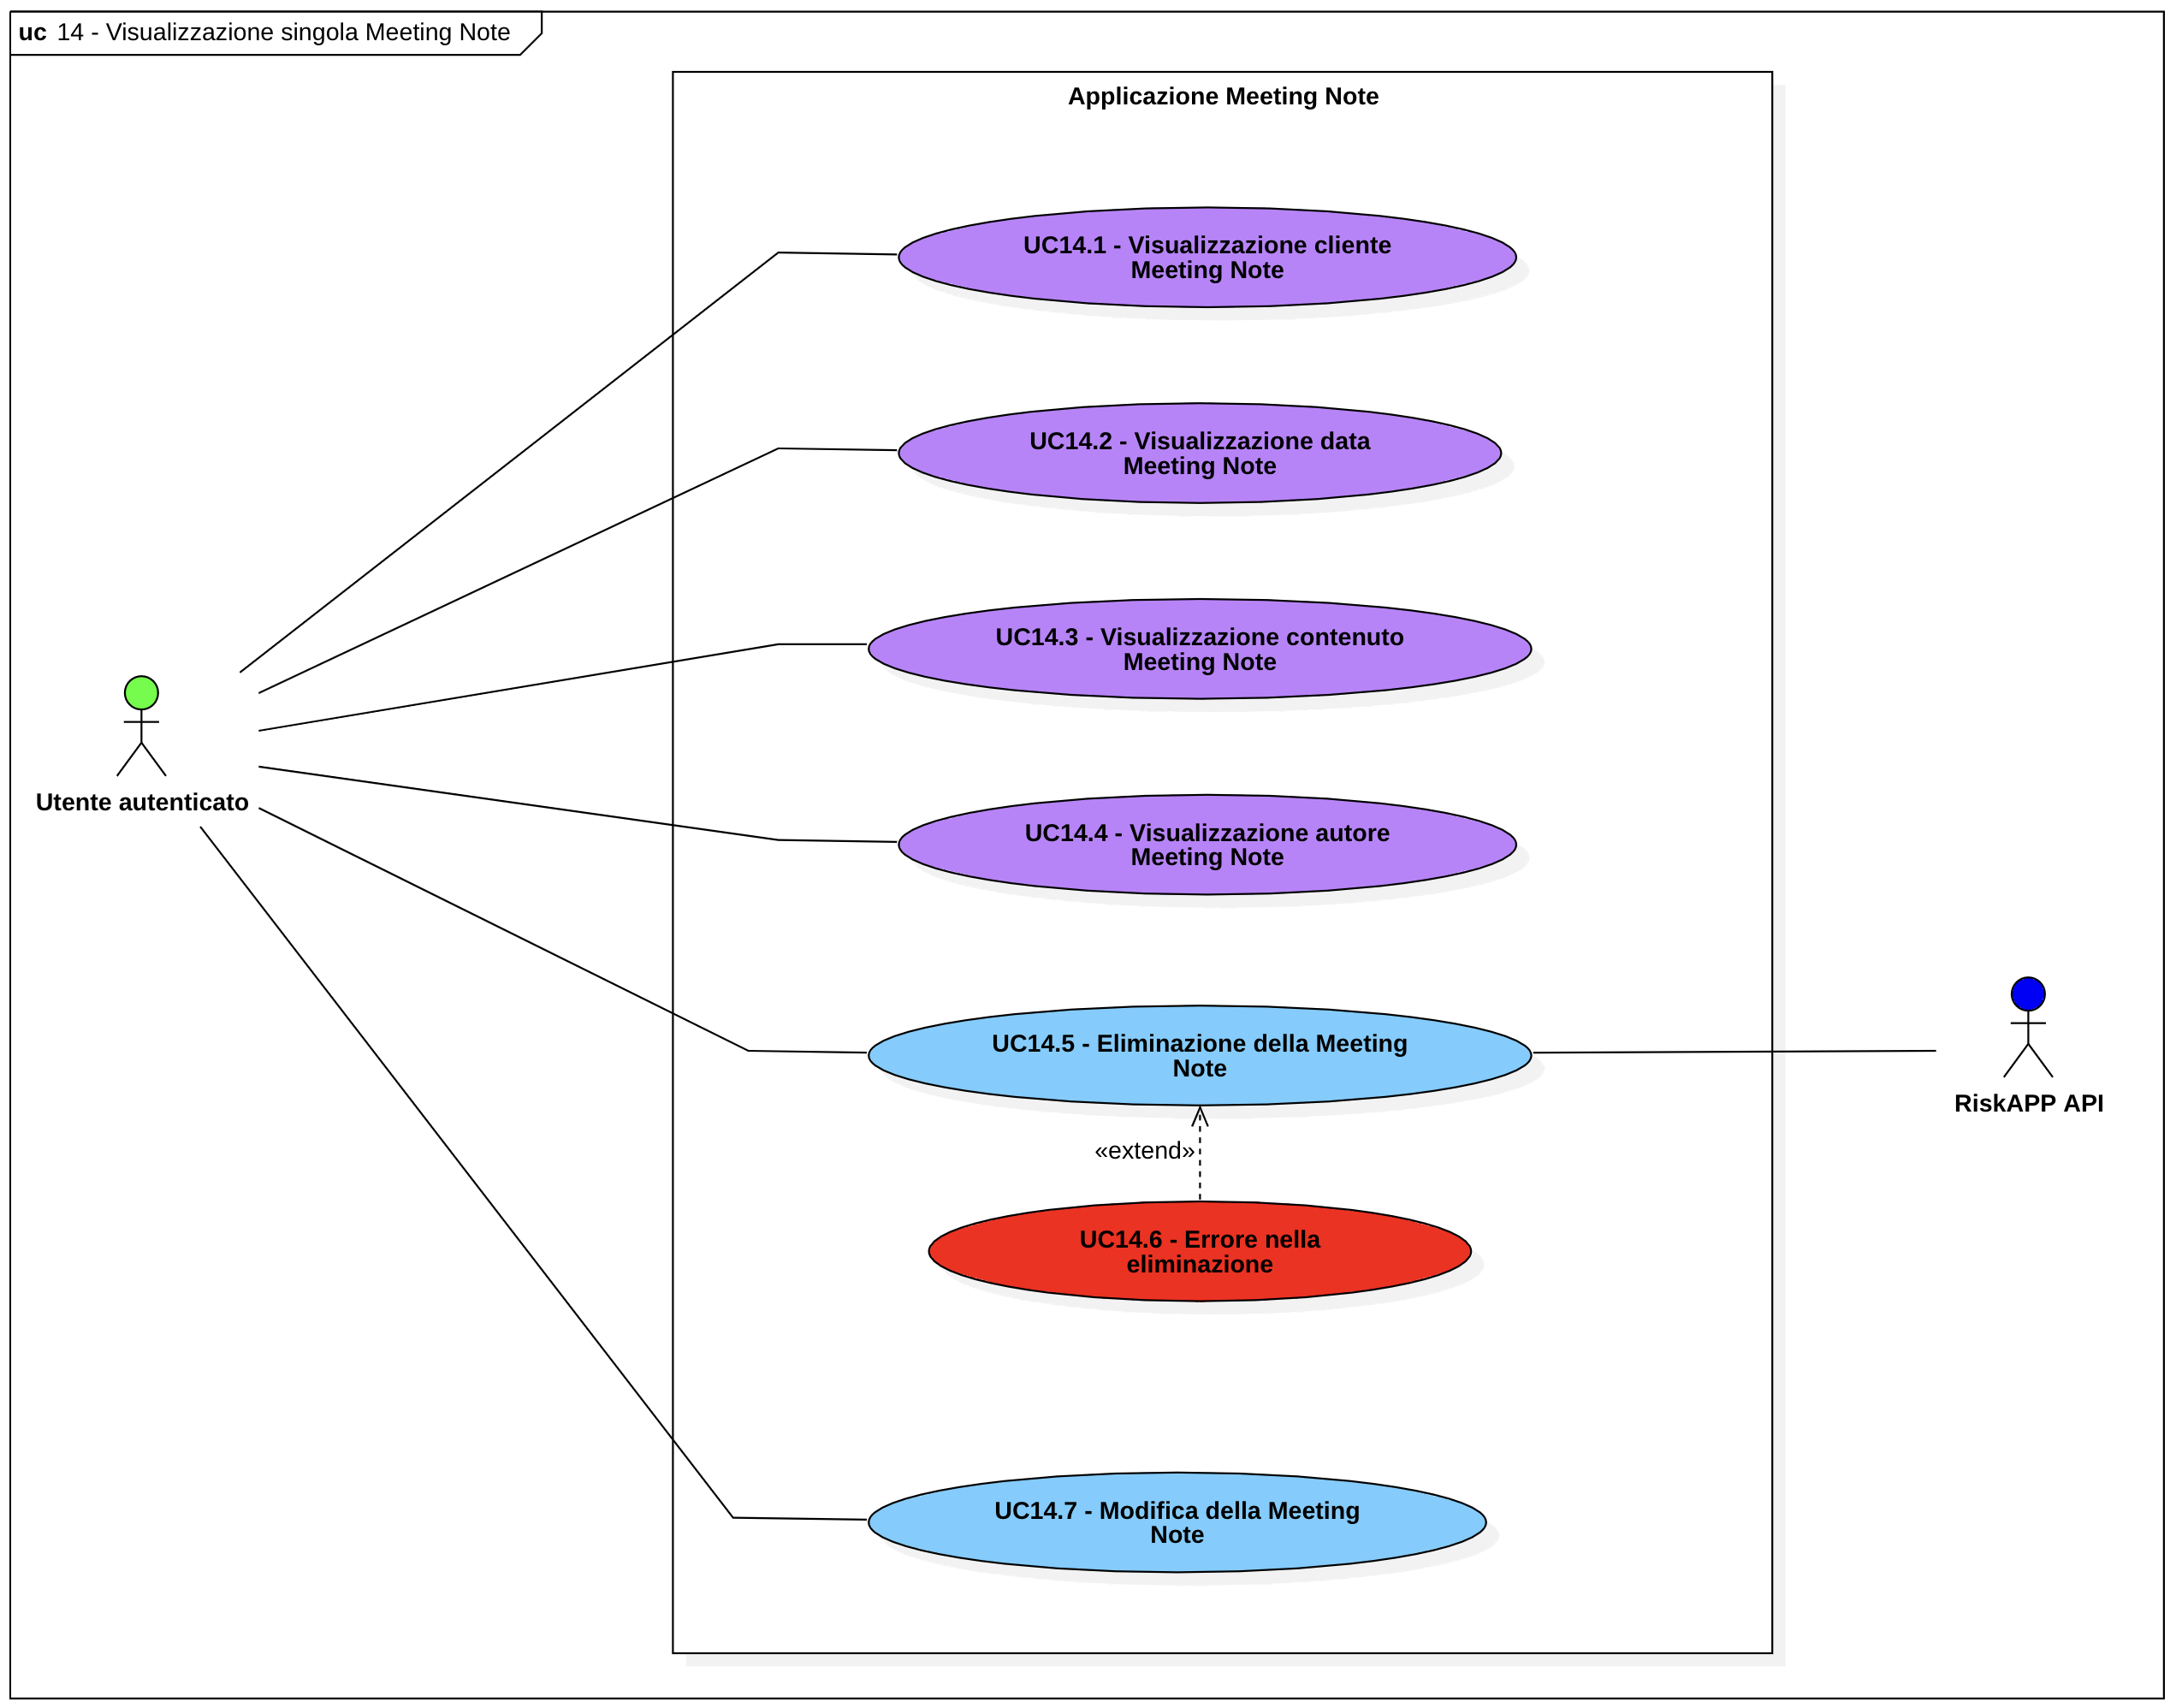
\includegraphics[width=1.0\columnwidth]{usecase/6-uc} 
    \caption{Use Case - Visualizzazione singola Meeting Note}
    \label{fig:uc-meetingnote-details}
\end{figure}

\begin{usecase}{14.1}{Visualizzazione cliente Meeting Note}
    \usecasemainactors{Utente autenticato}
    \usecasepre{L'utente visualizza i dettagli di una singola \gls{meetingnote}\glsoccur}
    \usecasedesc{L'utente vuole visualizzare il \gls{cliente}\glsoccur di una \gls{meetingnote}\glsoccur.}
    \usecasepost{È visualizzabile il \gls{cliente}\glsoccur di una \gls{meetingnote}\glsoccur}
    \usecaseimg{\ref{fig:uc-meetingnote-details}}
    \label{UC14.1}
\end{usecase}

\begin{usecase}{14.2}{Visualizzazione data Meeting Note}
    \usecasemainactors{Utente autenticato}
    \usecasepre{L'utente visualizza i dettagli di una singola \gls{meetingnote}\glsoccur}
    \usecasedesc{L'utente vuole visualizzare la data di una \gls{meetingnote}\glsoccur.}
    \usecasepost{È visualizzabile la data di una \gls{meetingnote}\glsoccur}
    \usecaseimg{\ref{fig:uc-meetingnote-details}}
    \label{UC14.2}
\end{usecase}

\begin{usecase}{14.3}{Visualizzazione contenuto Meeting Note}
    \usecasemainactors{Utente autenticato}
    \usecasepre{L'utente visualizza i dettagli di una singola \gls{meetingnote}\glsoccur}
    \usecasedesc{L'utente vuole visualizzare il contenuto di una \gls{meetingnote}\glsoccur.}
    \usecasepost{È visualizzabile il contenuto di una \gls{meetingnote}\glsoccur}
    \usecaseimg{\ref{fig:uc-meetingnote-details}}
    \label{UC14.3}
\end{usecase}

\begin{usecase}{14.4}{Visualizzazione autore Meeting Note}
    \usecasemainactors{Utente autenticato}
    \usecasepre{L'utente visualizza i dettagli di una singola \gls{meetingnote}\glsoccur}
    \usecasedesc{L'utente vuole visualizzare l'autore di una \gls{meetingnote}\glsoccur.}
    \usecasepost{È visualizzabile l'autore di una \gls{meetingnote}\glsoccur}
    \usecaseimg{\ref{fig:uc-meetingnote-details}}
    \label{UC14.4}
\end{usecase}

\begin{usecase}{14.5}{Eliminazione della Meeting Note}
    \usecasemainactors{Utente autenticato}
    \usecasesecondaryactors{\emph{RiskAPP API}}
    \usecasepre{L'utente visualizza i dettagli di una singola \gls{meetingnote}\glsoccur}
    \usecasedesc{L'utente vuole eliminare la \gls{meetingnote}\glsoccur selezionata.}
    \usecasepost{La \gls{meetingnote}\glsoccur selezionata è stata eliminata}
    \usecasealt{Se l'eliminazione fallisce, si verifica \hyperref[UC14.6]{UC14.6}}
    \usecaseimg{\ref{fig:uc-meetingnote-details}}
    \label{UC14.5}
\end{usecase}

\begin{usecase}{14.6}{Errore nella eliminazione}
    \usecasemainactors{Utente autenticato}
    \usecasesecondaryactors{\emph{RiskAPP API}}
    \usecasepre{L'utente visualizza i dettagli di una singola \gls{meetingnote}\glsoccur}
    \usecasedesc{L'eliminazione della \gls{meetingnote}\glsoccur selezionata fallisce e l'utente viene informato dell'errore; le motivazioni possono essere le seguenti:
        \begin{itemize}
            \item il sistema non è raggiungibile;
            \item token di autenticazione scaduto;
            \item connessione ad internet assente.
        \end{itemize}}
    \usecasepost{La \gls{meetingnote}\glsoccur selezionata non è stata eliminata}
    \usecaseimg{\ref{fig:uc-meetingnote-details}}
    \label{UC14.6}
\end{usecase}

\begin{usecase}{14.7}{Modifica della Meeting Note}
    \usecasemainactors{Utente autenticato}
    \usecasepre{L'utente visualizza i dettagli di una singola \gls{meetingnote}\glsoccur}
    \usecasedesc{L'utente vuole modificare la \gls{meetingnote}\glsoccur selezionata.}
    \usecasepost{La \gls{meetingnote}\glsoccur selezionata è stata modificata}
    \usecaseimg{\ref{fig:uc-meetingnote-details}}
    \label{UC14.7}
\end{usecase}

\begin{figure}[!h] 
    \centering 
    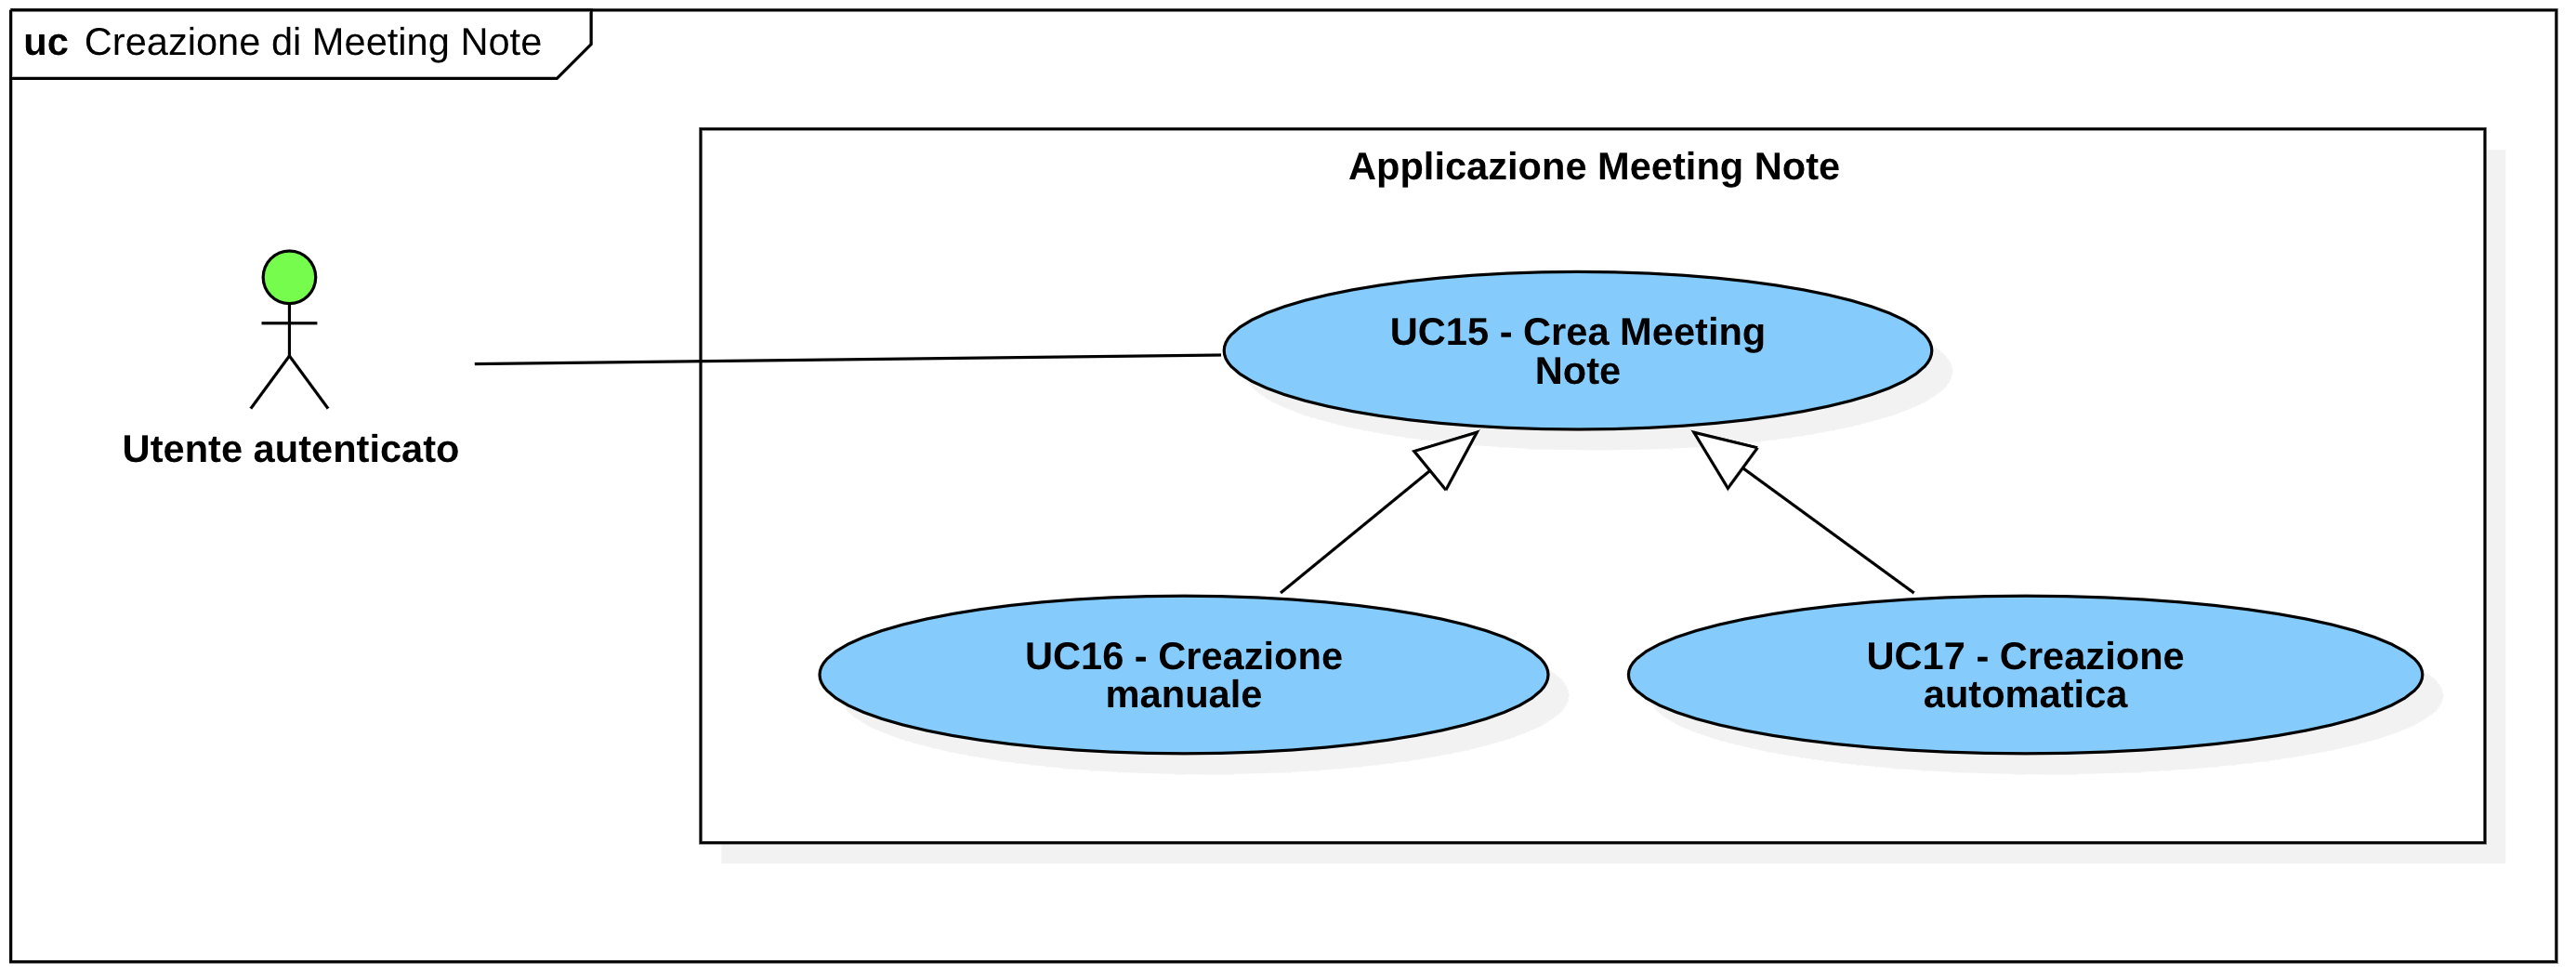
\includegraphics[width=1.0\columnwidth]{usecase/7-uc} 
    \caption{Use Case - Creazione Meeting Note}
    \label{fig:uc-meetingnote-create}
\end{figure}

\begin{usecase}{15}{Crea Meeting Note}
    \usecasemainactors{Utente autenticato}
    \usecasepre{L'utente è autenticato nel sistema}
    \usecasedesc{L'utente vuole creare una nuova \gls{meetingnote}\glsoccur.}
    \usecasepost{Una nuova \gls{meetingnote}\glsoccur è stata creata}
    \usecaseimg{\ref{fig:uc-meetingnote-create}}
    \label{UC15}
\end{usecase}

\begin{usecase}{16}{Creazione manuale}
    \usecasemainactors{Utente autenticato}
    \usecasepre{L'utente è autenticato nel sistema}
    \usecasedesc{L'utente vuole creare manualmente una nuova \gls{meetingnote}\glsoccur.}
    \usecasepost{Una nuova \gls{meetingnote}\glsoccur è stata creata manualmente}
    \usecaseimg{\ref{fig:uc-meetingnote-create}}
    \label{UC16}
\end{usecase}

\begin{usecase}{17}{Creazione automatica}
    \usecasemainactors{Utente autenticato}
    \usecasepre{L'utente è autenticato nel sistema}
    \usecasedesc{L'utente vuole creare automaticamente una nuova \gls{meetingnote}\glsoccur.}
    \usecasepost{Una nuova \gls{meetingnote}\glsoccur è stata creata automaticamente}
    \usecaseimg{\ref{fig:uc-meetingnote-create}}
    \label{UC17}
\end{usecase}

\begin{figure}[!h] 
    \centering 
    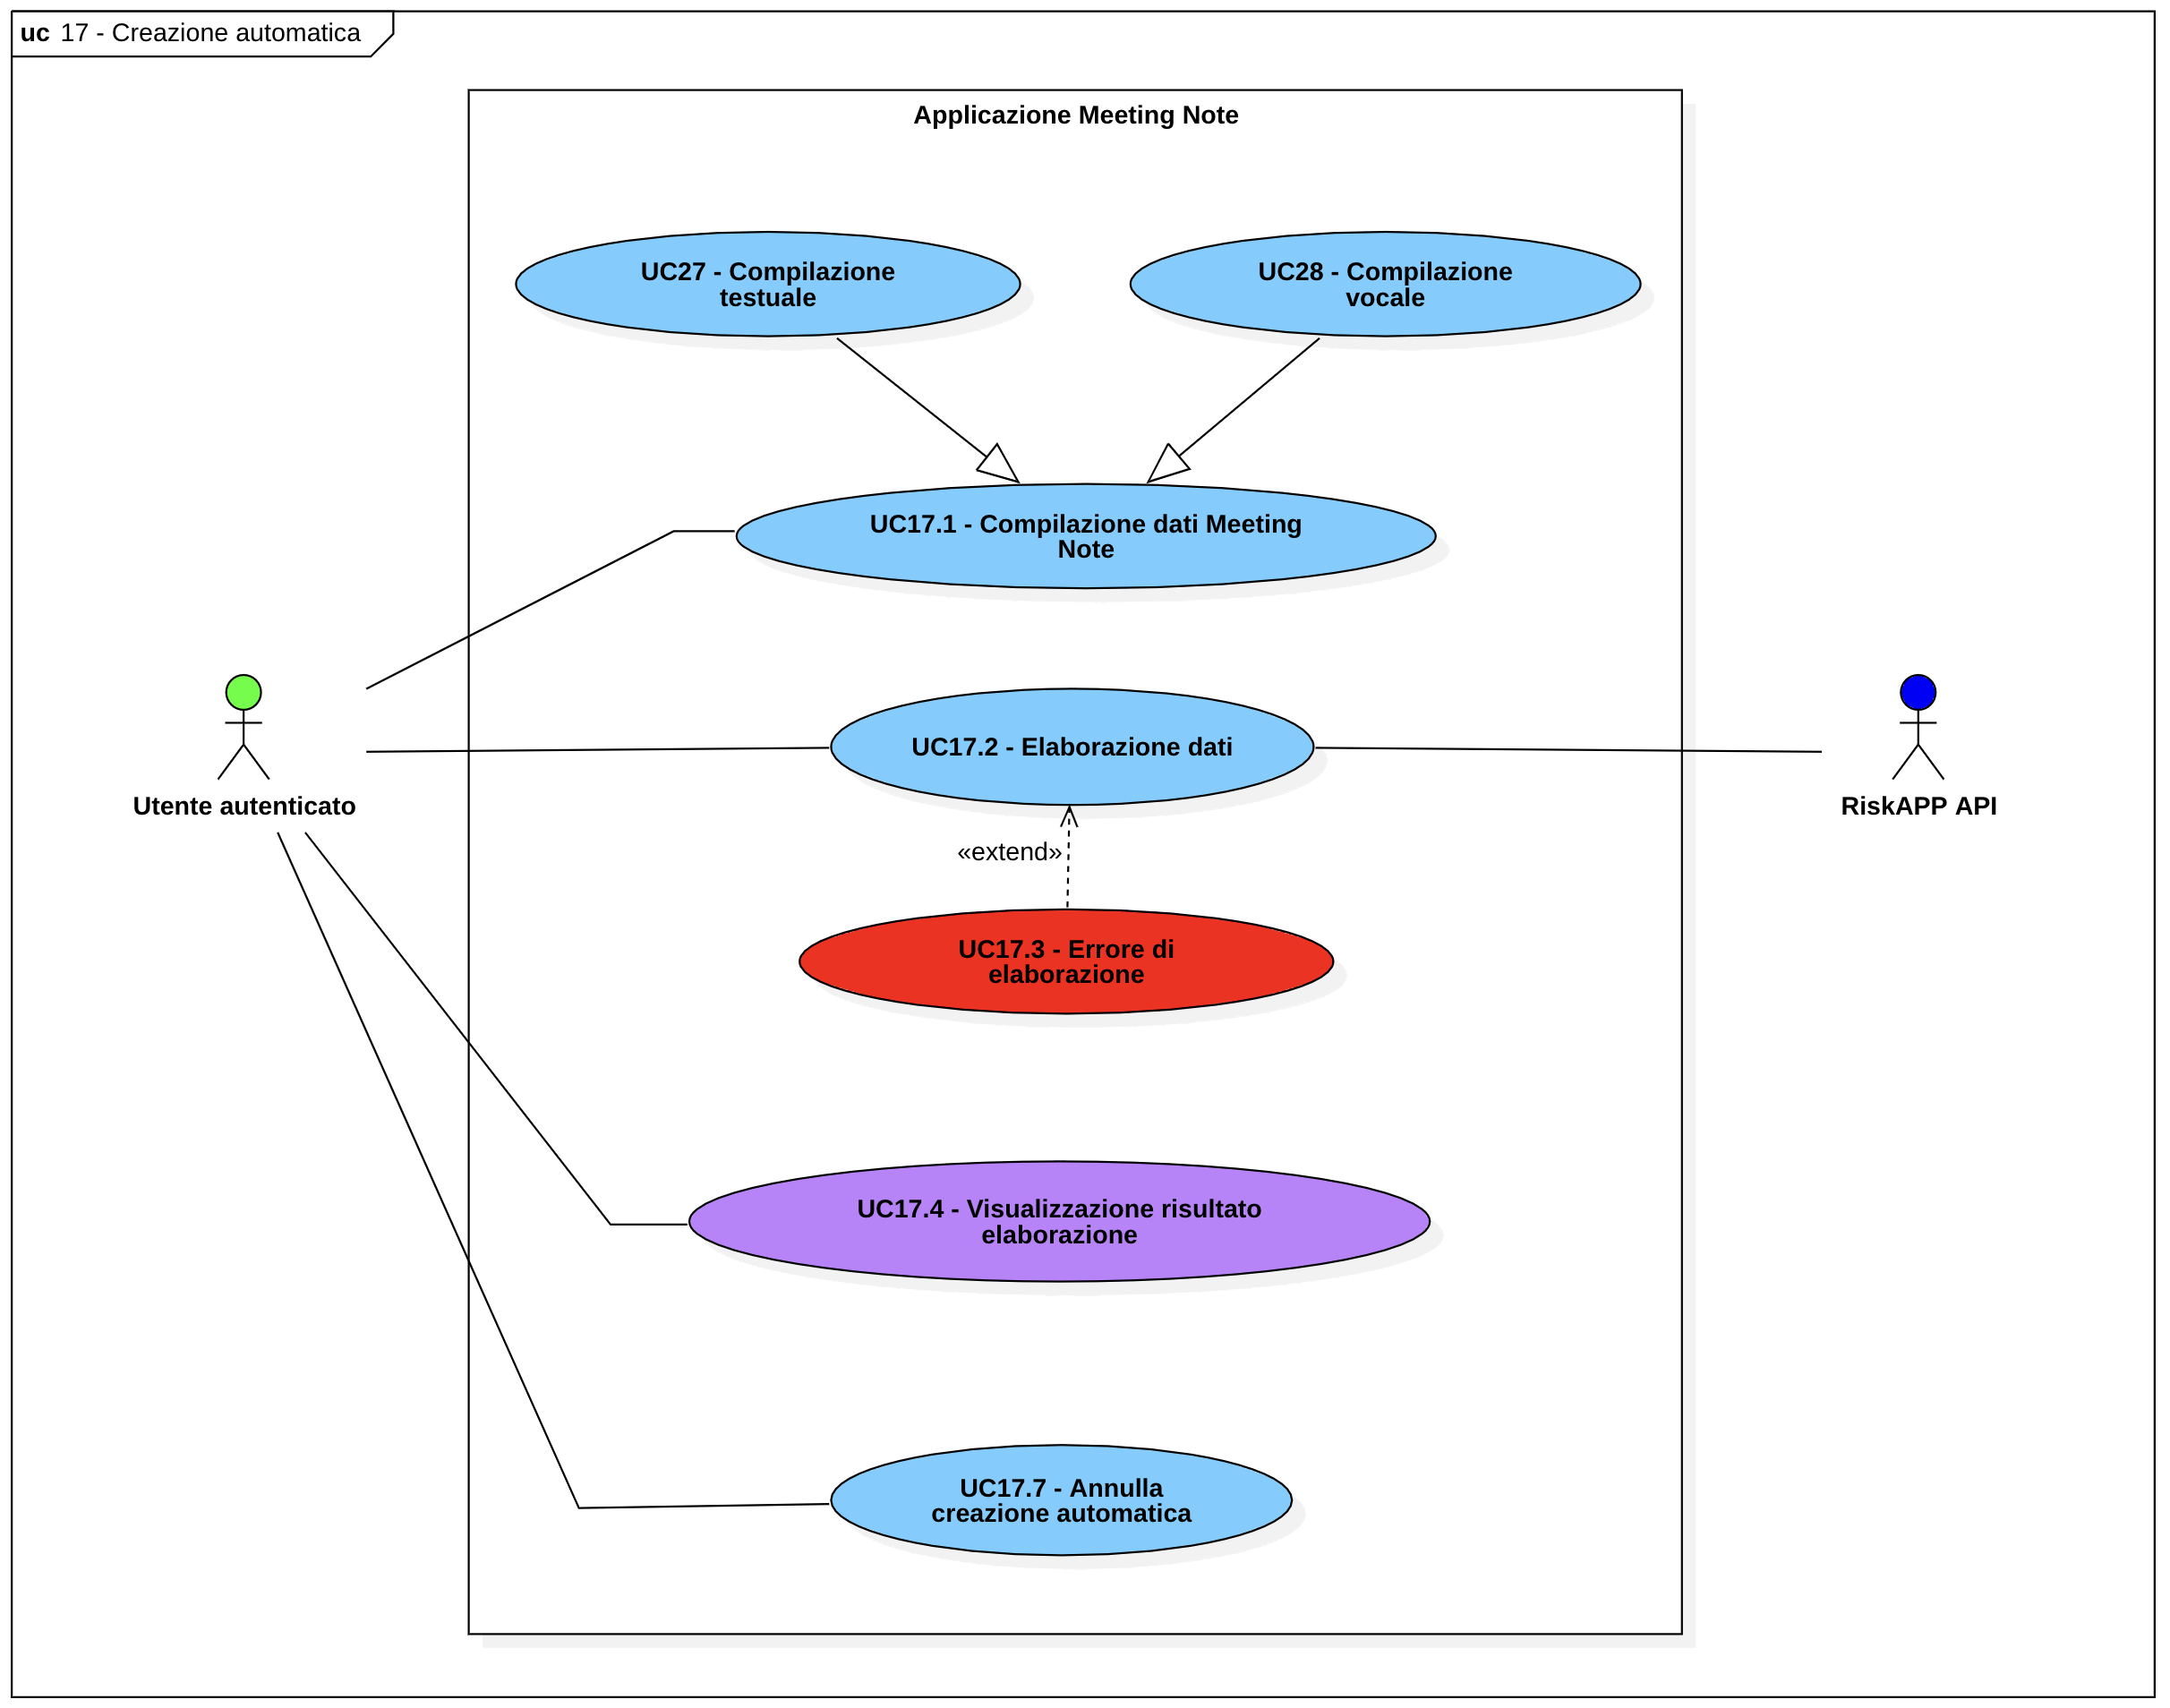
\includegraphics[width=1.0\columnwidth]{usecase/9-uc} 
    \caption{Use Case - Creazione automatica}
    \label{fig:uc-meetingnote-create-automatic}
\end{figure}

\begin{usecase}{17.1}{Compilazione dati Meeting Note}
    \usecasemainactors{Utente autenticato}
    \usecasepre{L'utente vuole creare automaticamente una \gls{meetingnote}\glsoccur}
    \usecasedesc{L'utente compila i dati necessari per la creazione automatica di una \gls{meetingnote}\glsoccur sotto forma di una descrizione testuale.}
    \usecasepost{È stato scritto una breve descrizione testuale con i dati necessari per la creazione automatica di una \gls{meetingnote}\glsoccur}
    \usecaseimg{\ref{fig:uc-meetingnote-create-automatic}}
    \label{UC17.1}
\end{usecase}

\begin{usecase}{17.2}{Elaborazione dati}
    \usecasemainactors{Utente autenticato}
    \usecasesecondaryactors{\emph{RiskAPP API}}
    \usecasepre{L'utente ha compilato i dati necessari per la creazione automatica di una \gls{meetingnote}\glsoccur}
    \usecasedesc{Il testo viene elaborato da una algoritmo di \gls{iag}\glsoccur per estrapolare i dati (cliente, data e contenuto) per la creazione automatica di una \gls{meetingnote}\glsoccur.}
    \usecasepost{I dati (cliente, data e contenuto) per la creazione automatica di una \gls{meetingnote}\glsoccur sono stati estrapolati}
    \usecasealt{Se l'elaborazione fallisce, si verifica \hyperref[UC17.3]{UC17.3}}
    \usecaseimg{\ref{fig:uc-meetingnote-create-automatic}}
    \label{UC17.2}
\end{usecase}

\begin{usecase}{17.3}{Errore elaborazione dati}
    \usecasemainactors{Utente autenticato}
    \usecasesecondaryactors{\emph{RiskAPP API}}
    \usecasepre{L'utente ha compilato i dati necessari per la creazione automatica di una \gls{meetingnote}\glsoccur}
    \usecasedesc{L'elaborazione dei dati per la creazione di una \gls{meetingnote}\glsoccur fallisce e l'utente viene informato dell'errore; le motivazioni possono essere le seguenti:
        \begin{itemize}
            \item l'algoritmo non è stato in grado di estrapolare i dati;
            \item il sistema non è raggiungibile;
            \item token di autenticazione scaduto;
            \item connessione ad internet assente.
        \end{itemize}}
    \usecasepost{I dati per la creazione automatica di una \gls{meetingnote}\glsoccur non sono stati estrapolati}
    \usecaseimg{\ref{fig:uc-meetingnote-create-automatic}}
    \label{UC17.3}
\end{usecase}

\begin{usecase}{17.4}{Visualizzazione risultato elaborazione}
    \usecasemainactors{Utente autenticato}
    \usecasepre{L'algoritmo ha estrapolato i dati per la creazione di una \gls{meetingnote}\glsoccur}
    \usecasedesc{L'utente vuole visualizzare i dati estrapolati dall'algoritmo per la creazione automatica di una \gls{meetingnote}\glsoccur, per accertarsi della loro correttezza.}
    \usecasepost{Sono visualizzabili i dati estrapolati dall'algoritmo per la creazione di una \gls{meetingnote}\glsoccur}
    \usecaseimg{\ref{fig:uc-meetingnote-create-automatic}}
    \label{UC17.4}
\end{usecase}

\newpage

\begin{figure}[!h] 
    \centering 
    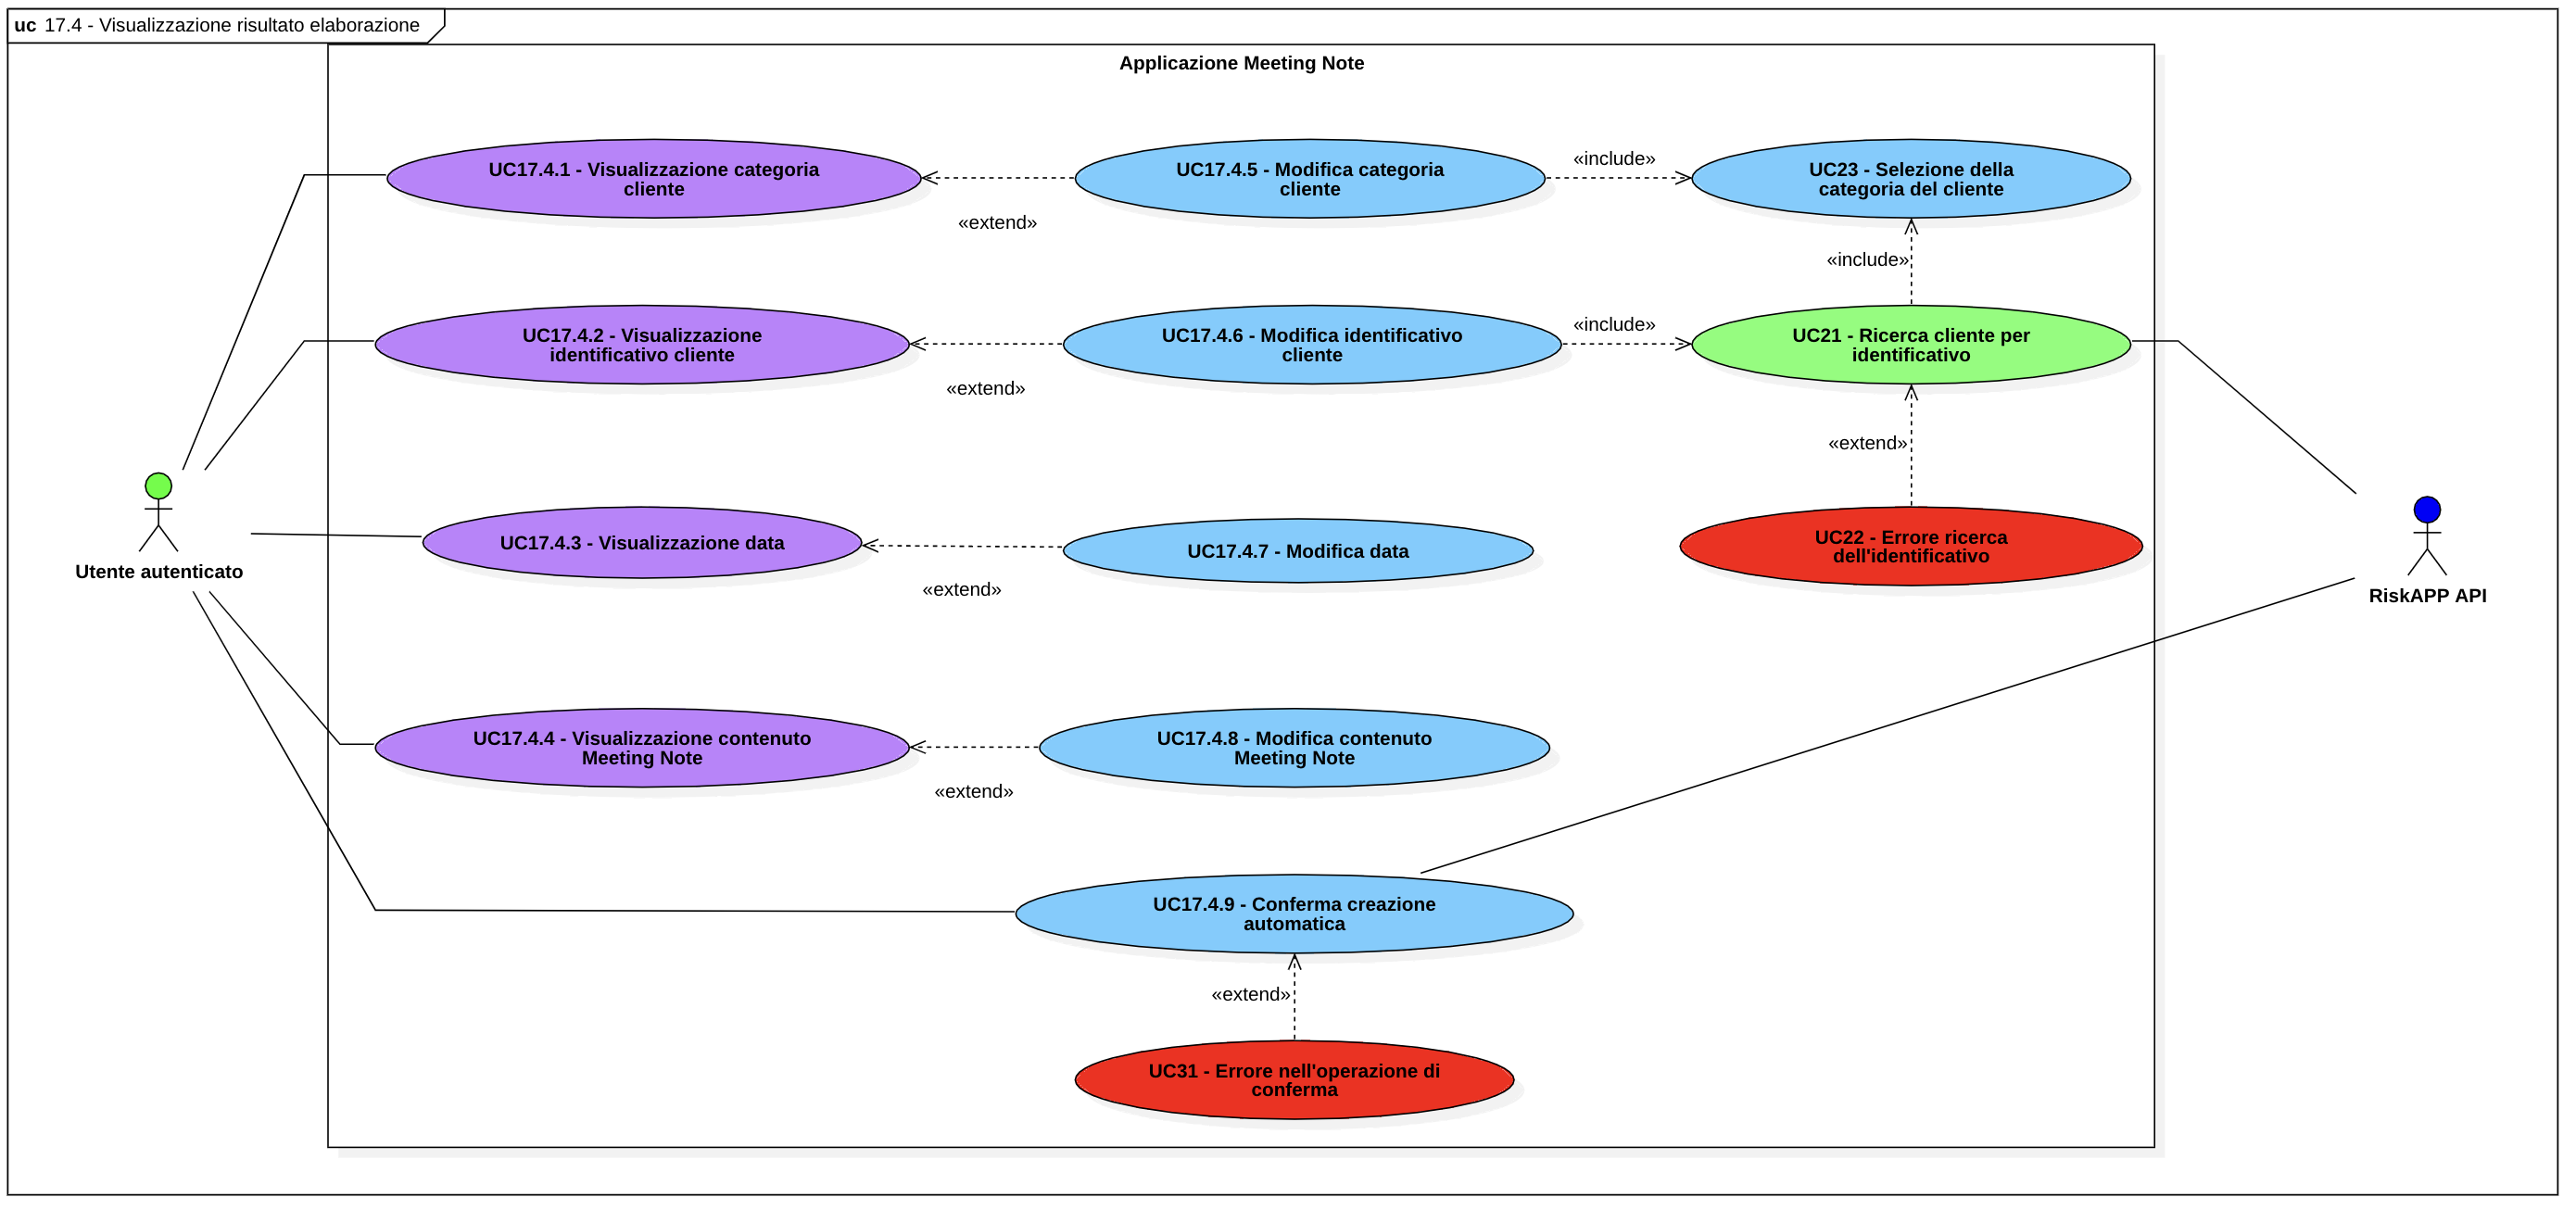
\includegraphics[width=1.0\columnwidth]{usecase/10-uc} 
    \caption{Use Case - Visualizzazione risultato elaborazione}
    \label{fig:uc-meetingnote-create-automatic-result}
\end{figure}

\begin{usecase}{17.4.1}{Visualizzazione categoria cliente}
    \usecasemainactors{Utente autenticato}
    \usecasepre{L'utente visualizza i dati estrapolati dall'algoritmo}
    \usecasedesc{L'utente vuole visualizzare la categoria del \gls{cliente}\glsoccur estrapolato}
    \usecasepost{È visualizzabile la categoria del \gls{cliente}\glsoccur estrapolato}
    \usecaseimg{\ref{fig:uc-meetingnote-create-automatic-result}}
    \label{UC17.4.1}
\end{usecase}

\begin{usecase}{17.4.2}{Visualizzazione identificativo cliente}
    \usecasemainactors{Utente autenticato}
    \usecasepre{L'utente visualizza i dati estrapolati dall'algoritmo}
    \usecasedesc{L'utente vuole visualizzare del \gls{cliente}\glsoccur estrapolato}
    \usecasepost{È visualizzabile l'identificativo del \gls{cliente}\glsoccur estrapolato}
    \usecaseimg{\ref{fig:uc-meetingnote-create-automatic-result}}
    \label{UC17.4.2}
\end{usecase}

\begin{usecase}{17.4.3}{Visualizzazione data}
    \usecasemainactors{Utente autenticato}
    \usecasepre{L'utente visualizza i dati estrapolati dall'algoritmo}
    \usecasedesc{L'utente vuole visualizzare la data estrapolata}
    \usecasepost{È visualizzabile la data estrapolata}
    \usecaseimg{\ref{fig:uc-meetingnote-create-automatic-result}}
    \label{UC17.4.3}
\end{usecase}

\begin{usecase}{17.4.4}{Visualizzazione il contenuto Meeting Note}
    \usecasemainactors{Utente autenticato}
    \usecasepre{L'utente visualizza i dati estrapolati dall'algoritmo}
    \usecasedesc{L'utente vuole visualizzare il contenuto estrapolato}
    \usecasepost{È visualizzabile il contenuto estrapolato}
    \usecaseimg{\ref{fig:uc-meetingnote-create-automatic-result}}
    \label{UC17.4.4}
\end{usecase}

\begin{usecase}{17.4.5}{Modifica categoria cliente}
    \usecasemainactors{Utente autenticato}
    \usecasepre{L'utente visualizza la categoria del \gls{cliente}\glsoccur estrapolato}
    \usecasedesc{L'utente modifica la categoria del \gls{cliente}\glsoccur}
    \usecasepost{La categoria del \gls{cliente}\glsoccur è stato modificato}
    \usecaseimg{\ref{fig:uc-meetingnote-create-automatic-result}}
    \label{15.4.5}
\end{usecase}

\begin{usecase}{17.4.6}{Modifica identificativo cliente}
    \usecasemainactors{Utente autenticato}
    \usecasepre{L'utente visualizza l'identificativo del \gls{cliente}\glsoccur estrapolato}
    \usecasedesc{L'utente modifica l'identificativo del \gls{cliente}\glsoccur}
    \usecasepost{L'identificativo del \gls{cliente}\glsoccur è stato modificato}
    \usecaseimg{\ref{fig:uc-meetingnote-create-automatic-result}}
    \label{15.4.6}
\end{usecase}

\begin{usecase}{17.4.7}{Modifica data}
    \usecasemainactors{Utente autenticato}
    \usecasepre{L'utente visualizza la data estrapolata}
    \usecasedesc{L'utente modifica la data}
    \usecasepost{La data è stata modificata}
    \usecaseimg{\ref{fig:uc-meetingnote-create-automatic-result}}
    \label{15.4.7}
\end{usecase}

\begin{usecase}{17.4.8}{Modifica contenuto Meeting Note}
    \usecasemainactors{Utente autenticato}
    \usecasepre{L'utente visualizza il contenuto estrapolato}
    \usecasedesc{L'utente modifica il contenuto}
    \usecasepost{Il contenuto è stato modificato}
    \usecaseimg{\ref{fig:uc-meetingnote-create-automatic-result}}
    \label{15.4.8}
\end{usecase}

\begin{usecase}{17.4.9}{Conferma creazione automatica}
    \usecasemainactors{Utente autenticato}
    \usecasepre{L'utente vuole creare automaticamente una \gls{meetingnote}\glsoccur}
    \usecasedesc{L'utente conferma la creazione automatica di una \gls{meetingnote}\glsoccur.}
    \usecasepost{Una nuova \gls{meetingnote}\glsoccur è stata creata automaticamente}
    \usecasealt{Se la conferma fallisce, si verifica \hyperref[UC31]{UC31}}
    \usecaseimg{\ref{fig:uc-meetingnote-create-automatic-result}}
    \label{15.4.9}
\end{usecase}

\begin{usecase}{17.5}{Annulla creazione automatica}
    \usecasemainactors{Utente autenticato}
    \usecasepre{L'utente è in fase di creazione automatica di una \gls{meetingnote}\glsoccur}
    \usecasedesc{L'utente annulla la creazione automatica di una \gls{meetingnote}\glsoccur.}
    \usecasepost{Non è stata creata una nuova \gls{meetingnote}\glsoccur}
    \usecaseimg{\ref{fig:uc-meetingnote-create-automatic}}
    \label{UC17.5}
\end{usecase}

\begin{figure}[!h] 
    \centering 
    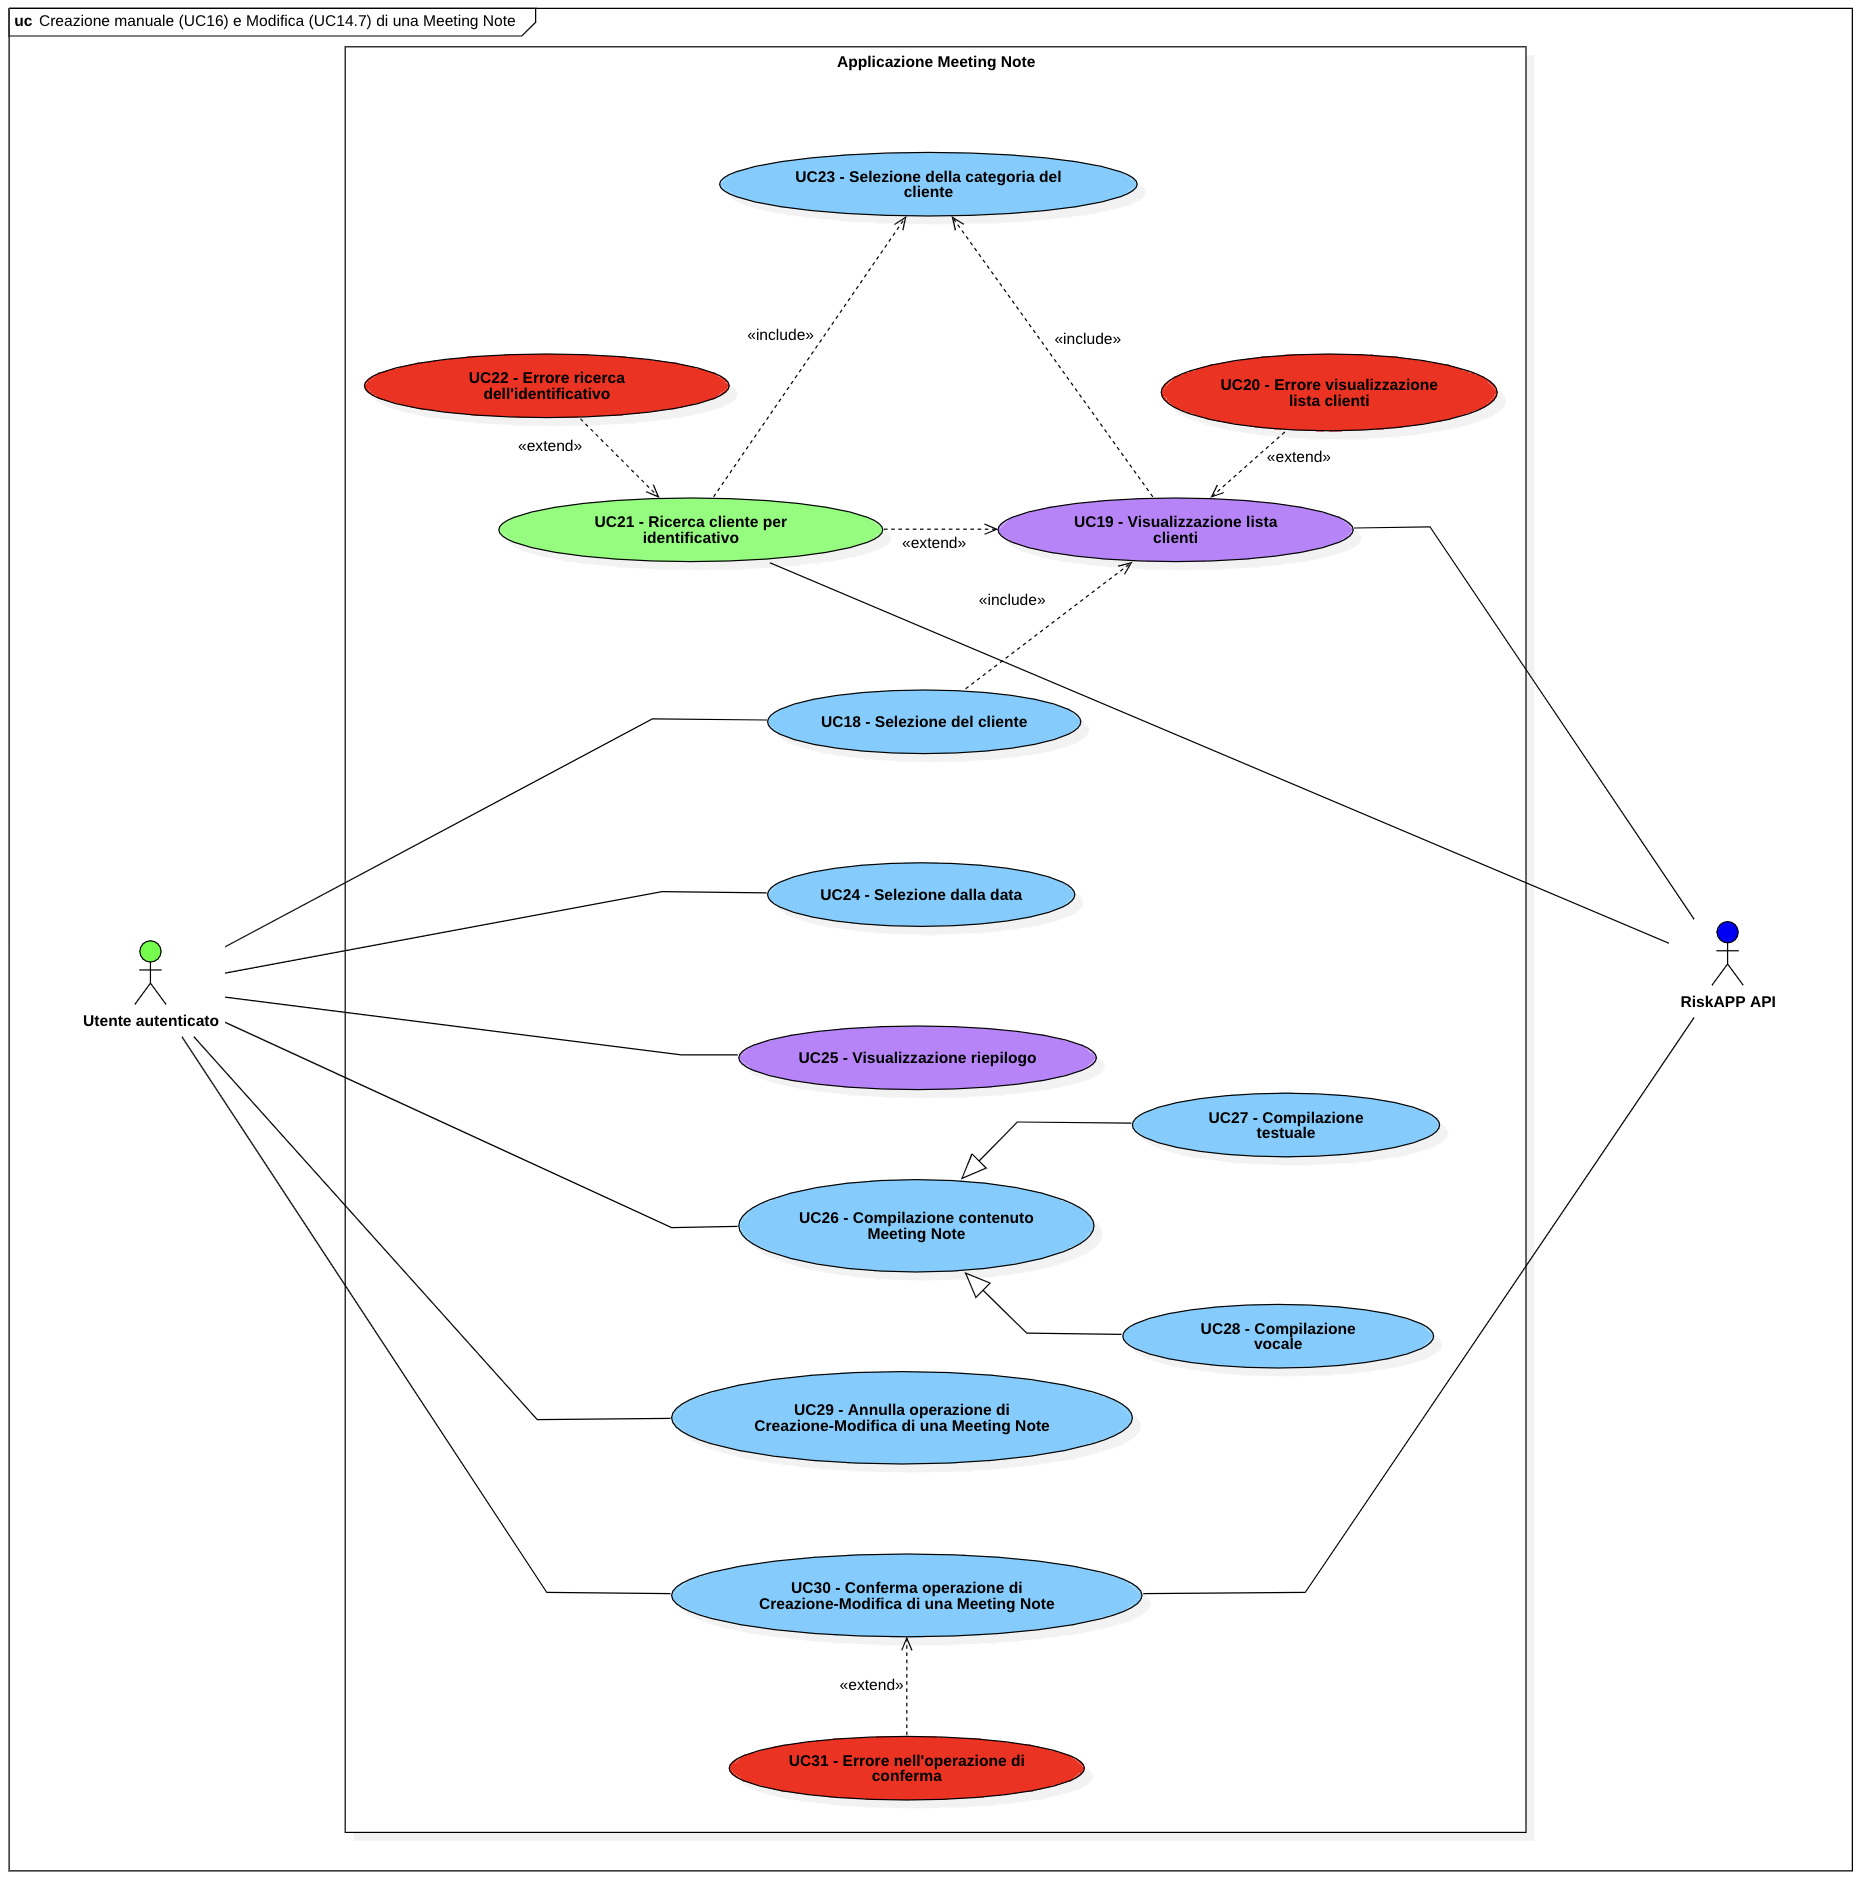
\includegraphics[width=1.0\columnwidth]{usecase/8-uc} 
    \caption{Use Case - Creazione manuale (\hyperref[UC16]{UC16}) e Modifica (\hyperref[UC14.7]{UC14.7}) di una Meeting Note}
    \label{fig:uc-meetingnote-create-manual}
\end{figure}

\newpage

\noindent Per la creazione manuale (\hyperref[UC16]{UC16}) e modifica (\hyperref[UC14.7]{UC14.7}) di una \gls{meetingnote}\glsoccur sono stati individuati i seguenti \glspl{usecase}\glsoccur, che sono in comune tra le due funzionalità sopra citate, in quanto condividono la stessa sequenza di azioni, e dunque di attori principali, secondari, precondizioni e postcondizioni.

\begin{usecase}{18}{Selezione del cliente}
    \usecasemainactors{Utente autenticato}
    \usecasepre{L'utente vuole creare manualmente o modificare una \gls{meetingnote}\glsoccur}
    \usecasedesc{L'utente deve selezionare un \gls{cliente}\glsoccur per la creazione o la modifica di una \gls{meetingnote}\glsoccur.}
    \usecasepost{Il \gls{cliente}\glsoccur è stato selezionato}
    \usecaseimg{\ref{fig:uc-meetingnote-create-manual}}
    \label{UC18}
\end{usecase}

\begin{usecase}{19}{Visualizzazione lista clienti}
    \usecasemainactors{Utente autenticato}
    \usecasesecondaryactors{\emph{RiskAPP API}}
    \usecasepre{L'utente ha selezionato la categoria del \gls{cliente}\glsoccur}
    \usecasedesc{L'utente vuole visualizzare la lista di tutti i \glspl{cliente}\glsoccur della categoria selezionata.}
    \usecasepost{È visualizzabile la lista dei \glspl{cliente}\glsoccur filtrata per categoria}
    \usecasealt{Se la visualizzazione fallisce, si verifica \hyperref[UC20]{UC20}}
    \usecaseimg{\ref{fig:uc-meetingnote-create-manual}}
    \label{UC19}
\end{usecase}

\begin{usecase}{20}{Errore visualizzazione lista clienti}
    \usecasemainactors{Utente autenticato}
    \usecasesecondaryactors{\emph{RiskAPP API}}
    \usecasepre{L'utente ha selezionato la categoria del \gls{cliente}\glsoccur}
    \usecasedesc{La visualizzazione della lista dei \glspl{cliente}\glsoccur fallisce e l'utente viene informato dell'errore; le motivazioni possono essere le seguenti:
        \begin{itemize}
            \item la lista è vuota;
            \item il sistema non è raggiungibile;
            \item token di autenticazione scaduto;
            \item connessione ad internet assente.
        \end{itemize}}
    \usecasepost{Non è visualizzabile la lista dei \glspl{cliente}\glsoccur filtrata per categoria}
    \usecaseimg{\ref{fig:uc-meetingnote-create-manual}}
    \label{UC20}
\end{usecase}

\newpage

\begin{usecase}{21}{Ricerca cliente per identificativo}
    \usecasemainactors{Utente autenticato}
    \usecasesecondaryactors{\emph{RiskAPP API}}
    \usecasepre{L'utente ha selezionato la categoria del \gls{cliente}\glsoccur}
    \usecasedesc{L'utente effettua una ricerca per identificativo del \gls{cliente}\glsoccur.}
    \usecasepost{L'identificativo del \gls{cliente}\glsoccur è stato trovato}
    \usecasealt{Se la ricerca fallisce, si verifica \hyperref[UC22]{UC22}}
    \usecaseimg{\ref{fig:uc-meetingnote-create-manual}}
    \label{UC21}
\end{usecase}

\begin{usecase}{22}{Errore ricerca dell'identificativo}
    \usecasemainactors{Utente autenticato}
    \usecasesecondaryactors{\emph{RiskAPP API}}
    \usecasepre{L'utente ha effettuato una ricerca per identificativo del \gls{cliente}\glsoccur}
    \usecasedesc{La ricerca dell'identificativo del \gls{cliente}\glsoccur fallisce e l'utente viene informato dell'errore; le motivazioni possono essere le seguenti:
        \begin{itemize}
            \item la lista risultante è vuota;
            \item il sistema non è raggiungibile;
            \item token di autenticazione scaduto;
            \item connessione ad internet assente.
        \end{itemize}}
    \usecasepost{L'identificativo del \gls{cliente}\glsoccur non è stato trovato}
    \usecaseimg{\ref{fig:uc-meetingnote-create-manual}}
    \label{UC22}
\end{usecase}

\begin{usecase}{23}{Selezione della categoria del cliente}
    \usecasemainactors{Utente autenticato}
    \usecasepre{L'utente è in fase di creazione o modifica}
    \usecasedesc{L'utente seleziona la categoria del \gls{cliente}\glsoccur per filtrare la lista dei \glspl{cliente}\glsoccur e/o la ricerca dell'identificativo.}
    \usecasepost{La categoria del \gls{cliente}\glsoccur è stata selezionata}
    \usecaseimg{\ref{fig:uc-meetingnote-create-manual}}
    \label{UC23}
\end{usecase}

\begin{usecase}{24}{Selezione della data}
    \usecasemainactors{Utente autenticato}
    \usecasepre{L'utente vuole creare manualmente o modificare una \gls{meetingnote}\glsoccur}
    \usecasedesc{L'utente deve selezionare una data, in cui è avvenuto l'incontro, per la creazione o la modifica di una \gls{meetingnote}\glsoccur.}
    \usecasepost{La data dell'incontro è stata selezionata}
    \usecaseimg{\ref{fig:uc-meetingnote-create-manual}}
    \label{UC24}
\end{usecase}

\begin{usecase}{25}{Visualizzazione riepilogo}
    \usecasemainactors{Utente autenticato}
    \usecasepre{L'utente ha selezionato un \gls{cliente}\glsoccur e una data}
    \usecasedesc{Viene visualizzato il riepilogo dei dati selezionati.}
    \usecasepost{È visualizzabile il riepilogo dei dati selezionati}
    \usecaseimg{\ref{fig:uc-meetingnote-create-manual}}
    \label{UC25}
\end{usecase}

\begin{figure}[!h] 
    \centering 
    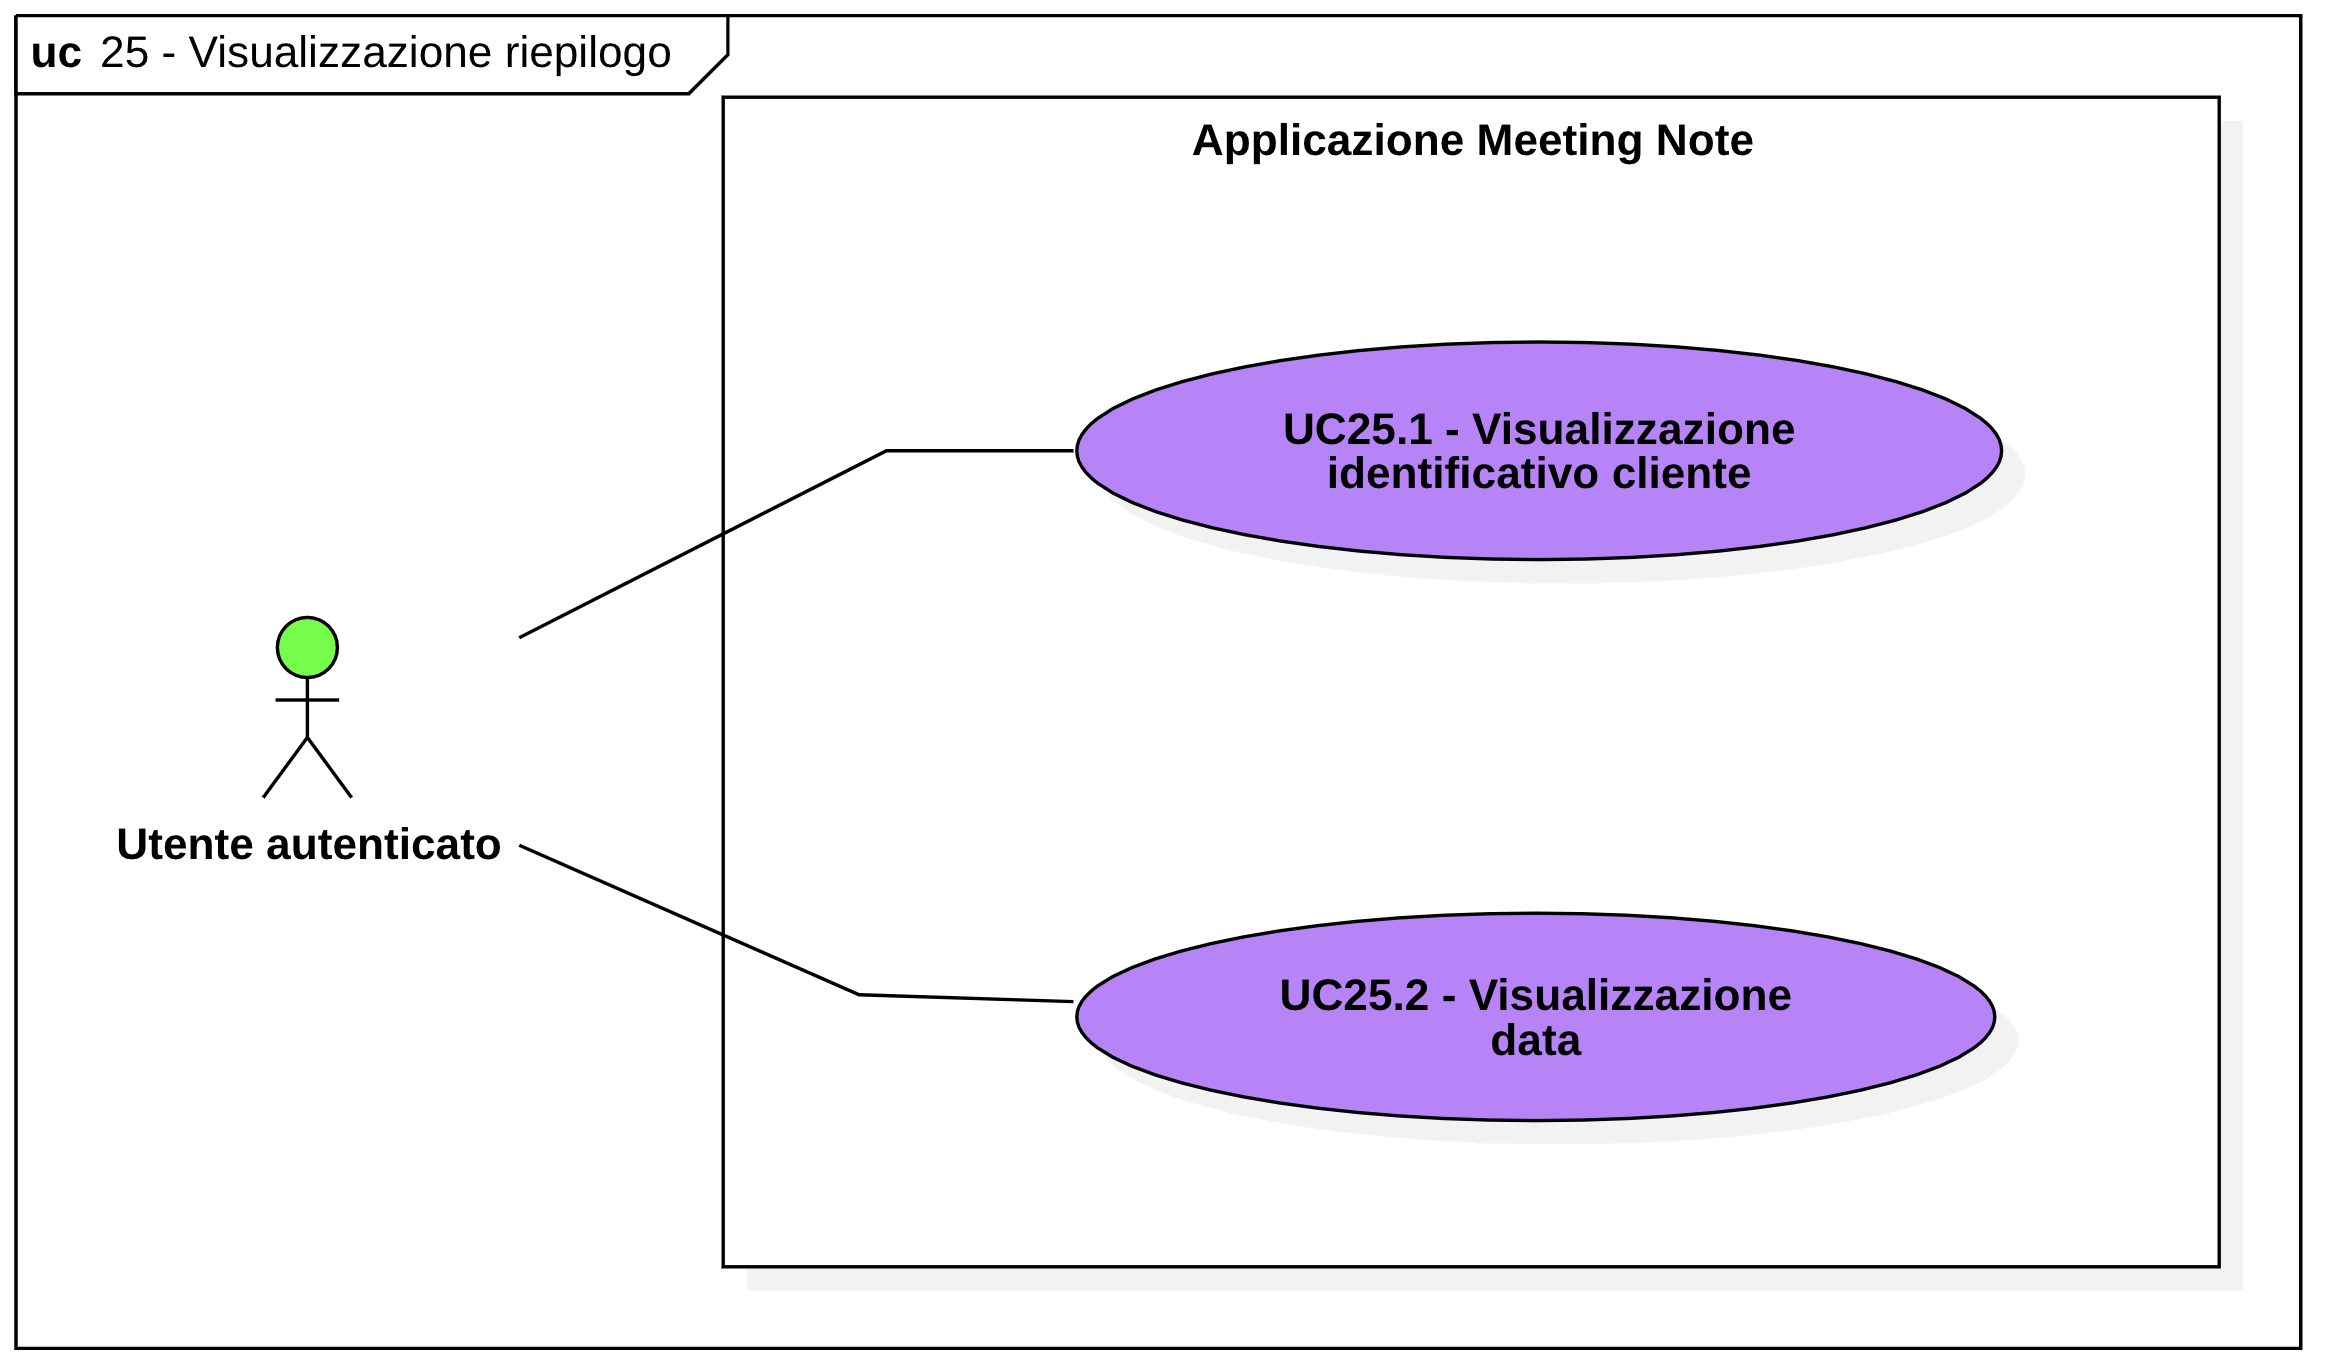
\includegraphics[width=1.0\columnwidth]{usecase/11-uc} 
    \caption{Use Case - Visualizzazione riepilogo}
    \label{fig:uc-meetingnote-create-manual-result}
\end{figure}

\begin{usecase}{25.1}{Visualizzazione identificativo cliente}
    \usecasemainactors{Utente autenticato}
    \usecasepre{L'utente visualizza il riepilogo}
    \usecasedesc{Viene visualizzato l'identificativo del \gls{cliente}\glsoccur selezionato.}
    \usecasepost{È visualizzabile l'identificativo del \gls{cliente}\glsoccur selezionato}
    \usecaseimg{\ref{fig:uc-meetingnote-create-manual-result}}
    \label{UC25.1}
\end{usecase}

\begin{usecase}{25.2}{Visualizzazione data}
    \usecasemainactors{Utente autenticato}
    \usecasepre{L'utente visualizza il riepilogo}
    \usecasedesc{Viene visualizzata la data selezionata.}
    \usecasepost{È visualizzabile la data selezionata}
    \usecaseimg{\ref{fig:uc-meetingnote-create-manual-result}}
    \label{UC25.2}
\end{usecase}

\begin{usecase}{26}{Compilazione contenuto Meeting Note}
    \usecasemainactors{Utente autenticato}
    \usecasepre{L'utente vuole creare manualmente o modificare una \gls{meetingnote}\glsoccur}
    \usecasedesc{L'utente deve compilare il contenuto della \gls{meetingnote}\glsoccur.}
    \usecasepost{Il contenuto della \gls{meetingnote}\glsoccur è compilato}
    \usecaseimg{\ref{fig:uc-meetingnote-create-manual}}
    \label{UC26}
\end{usecase}

\begin{usecase}{27}{Compilazione testuale}
    \usecasemainactors{Utente autenticato}
    \usecasepre{L'utente deve compilare il contenuto della \gls{meetingnote}\glsoccur}
    \usecasedesc{L'utente deve compilare il contenuto della \gls{meetingnote}\glsoccur con l'ausilio della tastiera.}
    \usecasepost{Il contenuto della \gls{meetingnote}\glsoccur è stato compilato con l'ausilio della tastiera}
    \usecaseimg{\ref{fig:uc-meetingnote-create-manual}}
    \label{UC27}
\end{usecase}

\begin{usecase}{28}{Compilazione vocale}
    \usecasemainactors{Utente autenticato}
    \usecasepre{L'utente deve compilare il contenuto della \gls{meetingnote}\glsoccur}
    \usecasedesc{L'utente deve compilare il contenuto della \gls{meetingnote}\glsoccur attraverso la dettatura vocale.}
    \usecasepost{Il contenuto della \gls{meetingnote}\glsoccur è stato compilato attraverso la dettatura vocale}
    \usecaseimg{\ref{fig:uc-meetingnote-create-manual}}
    \label{UC28}
\end{usecase}

\begin{usecase}{29}{Annulla operazione di Creazione-Modifica di una Meeting Note}
    \usecasemainactors{Utente autenticato}
    \usecasepre{L'utente ha selezionato: \gls{cliente}\glsoccur, data e compilato il contenuto della \gls{meetingnote}\glsoccur}
    \usecasedesc{L'utente vuole annullare l'operazione di creazione o modifica di una \gls{meetingnote}\glsoccur.}
    \usecasepost{L'operazione di creazione o modifica di una \gls{meetingnote}\glsoccur è annullata}
    \usecaseimg{\ref{fig:uc-meetingnote-create-manual}}
    \label{UC29}
\end{usecase}

\begin{usecase}{30}{Conferma operazione di Creazione-Modifica di una Meeting Note}
    \usecasemainactors{Utente autenticato}
    \usecasesecondaryactors{\emph{RiskAPP API}}
    \usecasepre{L'utente ha selezionato: \gls{cliente}\glsoccur, data e compilato il contenuto della \gls{meetingnote}\glsoccur}
    \usecasedesc{L'utente vuole confermare l'operazione di creazione o modifica di una \gls{meetingnote}\glsoccur.}
    \usecasepost{L'operazione di creazione o modifica di una \gls{meetingnote}\glsoccur è confermata}
    \usecasealt{Se la conferma fallisce, si verifica \hyperref[UC31]{UC31}}
    \usecaseimg{\ref{fig:uc-meetingnote-create-manual}}
    \label{UC30}
\end{usecase}

\begin{usecase}{31}{Errore nell'operazione di conferma}
    \usecasemainactors{Utente autenticato}
    \usecasesecondaryactors{\emph{RiskAPP API}}
    \usecasepre{L'utente ha confermato l'operazione di creazione o modifica di una \gls{meetingnote}\glsoccur}
    \usecasedesc{La conferma dell'operazione di creazione o modifica della \gls{meetingnote}\glsoccur fallisce e l'utente viene informato dell'errore; le motivazioni possono essere le seguenti:
        \begin{itemize}
            \item il sistema non è raggiungibile;
            \item token di autenticazione scaduto;
            \item connessione ad internet assente.
        \end{itemize}}
    \usecasepost{La conferma dell'operazione di creazione o modifica di una \gls{meetingnote}\glsoccur è fallita}
    \usecaseimg{\ref{fig:uc-meetingnote-create-manual}}
    \label{UC31}
\end{usecase}

\section{Tracciamento dei requisiti}

Da un'attenta analisi dei requisiti e dei casi d'uso effettuata sul progetto è stata stilata la tabella che traccia i requisiti.\\
Sono stati individuati diversi tipi di requisiti e si è quindi fatto utilizzo di un codice identificativo per distinguerli.\\
Il codice dei requisiti è così strutturato R(F/Q/V)(N/D/O) dove:
\begin{enumerate}
	\item[R =] requisito
    \item[F =] funzionale
    \item[Q =] qualitativo
    \item[V =] di vincolo
    \item[N =] obbligatorio (necessario)
    \item[D =] desiderabile
    \item[Z =] opzionale
\end{enumerate}

Di seguito sono riportate le tabelle che raccolgono, per tipologia, i requisiti individuati.\\
\begin{itemize}
    \item \textbf{Requisiti funzionali}: descrivono le funzionalità offerte dal prodotto software. Si faccia riferimento alle Tabelle \ref{tab:requisiti-funzionali-1}, \ref{tab:requisiti-funzionali-2}, \ref{tab:requisiti-funzionali-3}, \ref{tab:requisiti-funzionali-4};
    \item \textbf{Requisiti qualitativi}: descrivono le caratteristiche qualitative che il prodotto software deve possedere. Si faccia riferimento alla Tabella \ref{tab:requisiti-qualitativi};
    \item \textbf{Requisiti di vincolo}: descrivono i vincoli che il prodotto software deve rispettare. Si faccia riferimento alla Tabella \ref{tab:requisiti-vincolo}.
\end{itemize}

\noindent Nelle tabelle relative ai requisiti funzionali, alcuni di questi requisiti coinvolgono più \glspl{usecase}\glsoccur, la motivazione risiede nel fatto che essi ne modellano un comportamento comune, nello specifico si tratta di casi in cui vengono descritti scenari alternativi per la gestione di eccezioni.\\
Di seguito sono elencati, insieme ai relativi requisiti, i \gls{usecase}\glsoccur che, per questioni di leggibilità, non sono stai inseriti nelle tabelle:
\begin{itemize}
    \item \textbf{\hyperref[RFN-4]{RFN-4 }}: \hyperref[UC08.8]{UC08.8};
    \item \textbf{\hyperref[RFN-5]{RFN-5 }}: \hyperref[UC06]{UC06}, \hyperref[UC07.6]{UC07.6}, \hyperref[UC08.8]{UC08.8}, \hyperref[UC09]{UC09}, \hyperref[UC13]{UC13}, \hyperref[UC14.6]{UC14.6}, \hyperref[UC17.3]{UC17.3}, \hyperref[UC20]{UC20}, \hyperref[UC22]{UC22}, \hyperref[UC31]{UC31};
    \item \textbf{\hyperref[RFN-7]{RFN-7}}: \hyperref[UC06]{UC06}, \hyperref[UC07.6]{UC07.6}, \hyperref[UC08.8]{UC08.8}, \hyperref[UC09]{UC09}, \hyperref[UC13]{UC13}, \hyperref[UC14.6]{UC14.6}, \hyperref[UC17.3]{UC17.3}, \hyperref[UC20]{UC20}, \hyperref[UC22]{UC22}, \hyperref[UC31]{UC31};
    \item \textbf{\hyperref[RFN-13]{RFN-13}}: \hyperref[UC07.6]{UC07.6}, \hyperref[UC08.8]{UC08.8}, \hyperref[UC09]{UC09}, \hyperref[UC13]{UC13}, \hyperref[UC14.6]{UC14.6}, \hyperref[UC17.3]{UC17.3}, \hyperref[UC20]{UC20}, \hyperref[UC22]{UC22}, \hyperref[UC31]{UC31};
    \item \textbf{\hyperref[RFN-64]{RFN-64}}: \hyperref[UC22]{UC22}.
\end{itemize}

\begin{table}%
\caption{Tabella del tracciamento dei requisti funzionali - 1}
\label{tab:requisiti-funzionali-1}
\begin{tabularx}{\textwidth}{lXl}
\hline\hline
\textbf{Requisito} & \textbf{Descrizione} & \textbf{Use Case}\\
\hline
RFN-1 \label{RFN-1} & Il sistema permette di effettuare l'autenticazione & \hyperref[UC01]{UC01} \\
\hline
RFN-2 \label{RFN-2} & Il sistema permette di inserire le credenziali (\emph{username} e \emph{password}) per effettuare l'autenticazione & \hyperref[UC02]{UC02} \\
\hline
RFN-3 \label{RFN-3} & Il sistema permette il riconoscimento biometrico per effettuare l'autenticazione & \hyperref[UC03]{UC03} \\
\hline
% INSERIRE RFN CHE SPECIFICA IL FALLIMENTO DELL'AUTENTICAZIONE (IN TEORIA CI SONO ALTRI CASI SIMILI, DA SPECIFICARE ANALOGAMENTE)
RFN-4 \label{RFN-4} & Il sistema deve notificare l'utente in caso di inserimento di credenziali errate & \hyperref[UC04]{UC04} \\ % \hyperref[UC08.8]{UC08.8}
\hline
RFN-5 \label{RFN-5} & Il sistema deve notificare l'utente in caso in cui il sistema, ovvero la piattaforma \emph{RiskAPP} non sia raggiungibile & \hyperref[UC04]{UC04} \\ %, \hyperref[UC06]{UC06}, \hyperref[UC07.6]{UC07.6}, \hyperref[UC08.8]{UC08.8}, \hyperref[UC09]{UC09}, \hyperref[UC13]{UC13}, \hyperref[UC14.6]{UC14.6}, \hyperref[UC17.3]{UC17.3}, \hyperref[UC20]{UC20}, \hyperref[UC22]{UC22}, \hyperref[UC31]{UC31} 
\hline
RFN-6 \label{RFN-6} & Il sistema deve permettere all'utente, in caso in cui il riconoscimento biometrico fallisca, di poter inserire le credenziali manualmente & \hyperref[UC04]{UC04} \\
\hline
RFN-7 \label{RFN-7} & Il sistema deve notificare l'utente in caso di connessione internet assente & \hyperref[UC04]{UC04} \\ %, \hyperref[UC06]{UC06}, \hyperref[UC07.6]{UC07.6}, \hyperref[UC08.8]{UC08.8}, \hyperref[UC09]{UC09}, \hyperref[UC13]{UC13}, \hyperref[UC14.6]{UC14.6}, \hyperref[UC17.3]{UC17.3}, \hyperref[UC20]{UC20}, \hyperref[UC22]{UC22}, \hyperref[UC31]{UC31} 
\hline
RFN-8 \label{RFN-8} & Il sistema permette di visualizzare la lista di \emph{Meeting Note} & \hyperref[UC05]{UC05} \\
\hline
RFN-9 \label{RFN-9} & Il sistema permette di visualizzare i clienti di ciascuna \emph{Meeting Note} nella lista & \hyperref[UC05.1]{UC05.1} \\
\hline
RFN-10 \label{RFN-10} & Il sistema permette di visualizzare la data dell'incontro di ciascuna \emph{Meeting Note} nella lista & \hyperref[UC05.2]{UC05.2} \\
\hline
RFN-11 \label{RFN-11} & Il sistema permette di visualizzare parzialmente il contenuto di ciascuna \emph{Meeting Note} nella lista & \hyperref[UC05.3]{UC05.3} \\
\hline
RFN-12 \label{RFN-12} & Il sistema deve notificare l'utente in caso la lista di \emph{Meeting Note} sia vuota & \hyperref[UC06]{UC06} \\
\hline
RFN-13 \label{RFN-13} & Il sistema deve notificare l'utente in caso sia scaduto il token di autenticazione & \hyperref[UC06]{UC06} \\ % \hyperref[UC07.6]{UC07.6}, \hyperref[UC08.8]{UC08.8}, \hyperref[UC09]{UC09}, \hyperref[UC13]{UC13}, \hyperref[UC14.6]{UC14.6}, \hyperref[UC17.3]{UC17.3}, \hyperref[UC20]{UC20}, \hyperref[UC22]{UC22}, \hyperref[UC31]{UC31}
\hline
RFN-14 \label{RFN-14} & Il sistema permette di effettuare una ricerca nella lista di \emph{Meeting Note} & \hyperref[UC07]{UC07} \\
\hline
RFN-15 \label{RFN-15} & Il sistema permette di effettuare una ricerca nella lista di \emph{Meeting Note} per identificativo del cliente & \hyperref[UC07.1]{UC07.1} \\
\hline
RFN-16 \label{RFN-16} & Il sistema permette di selezionare la categoria del cliente in modo da effettuare una ricerca nella lista di \emph{Meeting Note} per identificativo del cliente & \hyperref[UC07.2]{UC07.2} \\
\hline
RFN-17 \label{RFN-17} & Il sistema permette di effettuare una ricerca nella lista di \emph{Meeting Note} per data & \hyperref[UC07.3]{UC07.3} \\
\hline
RFN-18 \label{RFN-18} & Il sistema permette di effettuare una ricerca nella lista di \emph{Meeting Note} per data singola & \hyperref[UC07.4]{UC07.4} \\
\hline
RFN-19 \label{RFN-19} & Il sistema permette di effettuare una ricerca nella lista di \emph{Meeting Note} per intervallo di date & \hyperref[UC07.5]{UC07.5} \\
\hline
RFN-20 \label{RFN-20} & Il sistema permette di notificare l'utente in caso la lista filtrata sia vuota & \hyperref[UC07.6]{UC07.6} \\
\hline
RFN-21 \label{RFN-21} & Il sistema permette di visualizzare i dati personali dell'utente & \hyperref[UC08]{UC08} \\
\hline
\end{tabularx}
\end{table}

\clearpage

\begin{table}%
\caption{Tabella del tracciamento dei requisti funzionali - 2}
\label{tab:requisiti-funzionali-2}
\begin{tabularx}{\textwidth}{lXl}
\hline\hline
\textbf{Requisito} & \textbf{Descrizione} & \textbf{Use Case}\\
\hline
RFN-22 \label{RFN-22} & Il sistema permette di visualizzare il nome dell'utente & \hyperref[UC08.1]{UC08.1} \\
\hline
RFN-23 \label{RFN-23} & Il sistema permette di visualizzare il cognome dell'utente & \hyperref[UC08.2]{UC08.2} \\
\hline
RFN-24 \label{RFN-24} & Il sistema permette di visualizzare la email dell'utente & \hyperref[UC08.3]{UC08.3} \\
\hline
RFN-25 \label{RFN-25} & Il sistema permette di visualizzare l'avatar dell'utente & \hyperref[UC08.4]{UC08.4} \\
\hline
RFN-26 \label{RFN-26} & Il sistema permette di effettuare il logout & \hyperref[UC08.5]{UC08.5} \\
\hline
RFN-27 \label{RFN-27} & Il sistema permette di abilitare il riconoscimento biometrico & \hyperref[UC08.6]{UC08.6} \\
\hline
RFN-28 \label{RFN-28} & Il sistema permette di confermare l'abilitazione del riconoscimento biometrico, inserendo le credenziali (\emph{username} e \emph{password}) & \hyperref[UC08.7]{UC08.7} \\
\hline
RFN-29 \label{RFN-29} & Il sistema permette di notificare l'utente in caso in cui la conferma per l'abilitazione del riconoscimento biometrico non vada a buon fine & \hyperref[UC08.8]{UC08.8} \\
\hline
RFN-30 \label{RFN-30} & Il sistema permette di notificare l'utente se la visualizzazione dei dati personali fallisce & \hyperref[UC09]{UC09} \\
\hline
RFN-31 \label{RFN-31} & Il sistema permette di ordinare la lista di \emph{Meeting Note} & \hyperref[UC10]{UC10} \\
\hline
RFN-32 \label{RFN-32} & Il sistema permette di ordinare la lista di \emph{Meeting Note} per data meno recente & \hyperref[UC11]{UC11} \\
\hline
RFN-33 \label{RFN-33} & Il sistema permette di ordinare la lista di \emph{Meeting Note} per data più recente & \hyperref[UC12]{UC12} \\
\hline
RFN-34 \label{RFN-34} & Il sistema permette di notificare l'utente se l'ordinamento della lista di \emph{Meeting Note} fallisce & \hyperref[UC13]{UC13} \\
\hline
RFN-35 \label{RFN-35} & Il sistema permette di visualizzare il contenuto integrale di una \emph{Meeting Note} selezionata & \hyperref[UC14]{UC14} \\
\hline
RFN-36 \label{RFN-36} & Il sistema permette di visualizzare l'identificativo del cliente di una \emph{Meeting Note} selezionata & \hyperref[UC14.1]{UC14.1} \\
\hline
% SCORDATO LA PARTITA IVA PER I CONTRAENTI (CLIENTI)
RFN-37 \label{RFN-37} & Il sistema permette di visualizzare la data dell'incontro di una \emph{Meeting Note} selezionata & \hyperref[UC14.2]{UC14.2} \\
\hline
RFN-38 \label{RFN-38} & Il sistema permette di visualizzare il contenuto dell'incontro di una \emph{Meeting Note} selezionata & \hyperref[UC14.3]{UC14.3} \\
\hline
RFN-39 \label{RFN-39} & Il sistema permette di visualizzare l'autore di una \emph{Meeting Note} selezionata & \hyperref[UC14.4]{UC14.4} \\
\hline
RFN-40 \label{RFN-40} & Il sistema permette di eliminare una \emph{Meeting Note} selezionata & \hyperref[UC14.5]{UC14.5} \\
\hline
RFN-41 \label{RFN-41} & Il sistema permette di notificare l'utente in caso in cui l'eliminazione di una \emph{Meeting Note} selezionata fallisca & \hyperref[UC14.6]{UC14.6} \\
\hline
RFN-42 \label{RFN-42} & Il sistema permette di modificare una \emph{Meeting Note} selezionata & \hyperref[UC14.7]{UC14.7} \\
\hline
\end{tabularx}
\end{table}

\clearpage

\begin{table}%
    \caption{Tabella del tracciamento dei requisti funzionali - 3}
    \label{tab:requisiti-funzionali-3}
    \begin{tabularx}{\textwidth}{lXl}
    \hline\hline
    \textbf{Requisito} & \textbf{Descrizione} & \textbf{Use Case}\\
    \hline
    RFN-43 \label{RFN-43} & Il sistema permette di effettuare la creazione di una \emph{Meeting Note} & \hyperref[UC15]{UC15} \\
    \hline
    RFN-44 \label{RFN-44} & Il sistema permette di effettuare la creazione manuale di una \emph{Meeting Note} & \hyperref[UC16]{UC16} \\
    \hline
    RFD-45 \label{RFD-45} & Il sistema permette di effettuare la creazione automatica di una \emph{Meeting Note} & \hyperref[UC17]{UC17} \\
    \hline
    RFD-46 \label{RFD-46} & Il sistema permette di compilare i dati (cliente, data e contenuto), sotto forma di una descrizione testuale, di una \emph{Meeting Note} per la creazione automatica & \hyperref[UC17.1]{UC17.1} \\
    \hline
    RFD-47 \label{RFD-47} & Il sistema permette di effettuare l'elaborazione del testo da parte di un algoritmo di \gls{iag}\glsoccur per l'estrapolazione dei dati (cliente, data e contenuto) & \hyperref[UC17.2]{UC17.2} \\
    \hline
    RFD-48 \label{RFD-48} & Il sistema permette di notificare l'utente in caso in cui l'elaborazione del testo non vada a buon fine & \hyperref[UC17.3]{UC17.3} \\
    \hline
    RFD-49 \label{RFD-49} & Il sistema permette di notificare l'utente in caso in cui l'algoritmo di elaborazione non è in grado di estrapolare, dal testo, i dati (cliente, data e contenuto) & \hyperref[UC17.3]{UC17.3} \\
    \hline
    RFD-50 \label{RFD-50} & Il sistema permette di visualizzare il risultato dell'elaborazione dei dati & \hyperref[UC17.4]{UC17.4} \\
    \hline
    RFD-51 \label{RFD-51} & Il sistema permette di visualizzare la categoria del cliente estrapolato & \hyperref[UC17.4.1]{UC17.4.1} \\
    \hline
    RFD-52 \label{RFD-52} & Il sistema permette di visualizzare l'identificativo del cliente estrapolato & \hyperref[UC17.4.2]{UC17.4.2} \\
    \hline
    RFD-53 \label{RFD-53} & Il sistema permette di visualizzare la data dell'incontro estrapolata & \hyperref[UC17.4.3]{UC17.4.3} \\
    \hline
    RFD-54 \label{RFD-54} & Il sistema permette di visualizzare il contenuto dell'incontro estrapolato & \hyperref[UC17.4.4]{UC17.4.4} \\
    \hline
    RFD-55 \label{RFD-55} & Il sistema permette di modificare la categoria del cliente estrapolato & \hyperref[UC17.4.5]{UC17.4.5} \\
    \hline
    RFD-56 \label{RFD-56} & Il sistema permette di modificare l'identificativo del cliente estrapolato & \hyperref[UC17.4.6]{UC17.4.6} \\
    \hline
    RFD-57 \label{RFD-57} & Il sistema permette di modificare la data dell'incontro estrapolata & \hyperref[UC17.4.7]{UC17.4.7} \\
    \hline
    RFD-58 \label{RFD-58} & Il sistema permette di modificare il contenuto dell'incontro estrapolato & \hyperref[UC17.4.8]{UC17.4.8} \\
    \hline
    RFD-59 \label{RFD-59} & Il sistema permette di confermare la creazione automatica & \hyperref[UC17.4.9]{UC17.4.9} \\
    \hline
    RFD-60 \label{RFD-60} & Il sistema permette di annullare l'operazione di creazione automatica & \hyperref[UC17.5]{UC17.5} \\
    \hline
\end{tabularx}
\end{table}

\clearpage

\begin{table}%
    \caption{Tabella del tracciamento dei requisti funzionali - 4}
    \label{tab:requisiti-funzionali-4}
    \begin{tabularx}{\textwidth}{lXl}
    \hline\hline
    \textbf{Requisito} & \textbf{Descrizione} & \textbf{Use Case}\\
    \hline
    RFN-61 \label{RFN-61} & Il sistema permette di selezionare il cliente per la creazione manuale di una \emph{Meeting Note} & \hyperref[UC18]{UC18} \\
    \hline
    RFN-62 \label{RFN-62} & Il sistema permette di visualizzare la lista dei clienti per la selezione & \hyperref[UC19]{UC19} \\
    \hline
    RFN-63 \label{RFN-63} & Il sistema permette di notificare l'utente in caso cui la visualizzazione della lista dei clienti fallisca & \hyperref[UC20]{UC20} \\
    \hline
    RFN-64 \label{RFN-64} & Il sistema deve notificare l'utente in caso la lista dei clienti sia vuota & \hyperref[UC20]{UC20} \\ % \hyperref[UC22]{UC22}
    \hline
    RFN-65 \label{RFN-65} & Il sistema deve permettere di ricercare un cliente nella lista per identificativo & \hyperref[UC21]{UC21} \\
    \hline
    RFN-66 \label{RFN-66} & Il sistema deve permettere di selezionare la categoria del cliente & \hyperref[UC23]{UC23} \\
    \hline
    RFN-67 \label{RFN-67} & Il sistema permette di selezionare la data per la creazione manuale di una \emph{Meeting Note} & \hyperref[UC24]{UC24} \\
    \hline
    RFN-68 \label{RFN-68} & Il sistema permette di visualizzare il riepilogo dei dati selezionati & \hyperref[UC25]{UC25} \\
    \hline
    RFN-69 \label{RFN-69} & Il sistema permette di visualizzare l'identificativo del cliente selezionato & \hyperref[UC25.1]{UC25.1} \\
    \hline
    RFN-70 \label{RFN-70} & Il sistema permette di visualizzare la data selezionata & \hyperref[UC25.2]{UC25.2} \\
    \hline
    RFN-71 \label{RFN-71} & Il sistema permette di compilare il contenuto della \emph{Meeting Note} & \hyperref[UC26]{UC26} \\
    \hline
    RFN-72 \label{RFN-72} & Il sistema permette di compilare il contenuto della \emph{Meeting Note} con l'ausilio della tastiera & \hyperref[UC27]{UC27} \\
    \hline
    RFN-73 \label{RFN-73} & Il sistema permette di compilare il contenuto della \emph{Meeting Note} con l'ausilio della dettatura vocale & \hyperref[UC28]{UC28} \\
    \hline
    RFN-74 \label{RFN-74} & Il sistema permette di annullare l'operazione di creazione o modifica di una \emph{Meeting Note} & \hyperref[UC29]{UC29} \\
    \hline
    RFN-75 \label{RFN-75} & Il sistema permette di confermare l'operazione di creazione o modifica di una \emph{Meeting Note} & \hyperref[UC30]{UC30} \\
    \hline
    RFN-76 \label{RFN-76} & Il sistema permette di notificare l'utente in caso in cui la conferma dell'operazione di creazione o modifica di una \emph{Meeting Note} non vada a buon fine & \hyperref[UC31]{UC31} \\
    \hline
\end{tabularx}
\end{table}

\begin{table}%
\caption{Tabella del tracciamento dei requisiti qualitativi}
\label{tab:requisiti-qualitativi}
\begin{tabularx}{\textwidth}{lXl}
\hline\hline
\textbf{Requisito} & \textbf{Descrizione} & \textbf{Fonte}\\
\hline
RQD-1 & Il sistema deve garantire il corretto funzionamento attraverso l'implementazione ed esecuzione di test & \hyperref[F01]{F01} \\
\hline
RQN-2 & Il codice prodotto deve essere disponibile su \gls{github}\glsoccur, nella repository aziendale  & Azienda \\
\hline
RQN-3 & Il codice prodotto deve essere documentato & Azienda \\
\hline
RQN-4 & L'applicazione deve soddisfare la proprietà di \gls{responsivita}\glsoccur del \emph{layout} & Azienda \\
\hline
\end{tabularx}
\end{table}%

\begin{table}%
\caption{Tabella del tracciamento dei requisiti di vincolo}
\label{tab:requisiti-vincolo}
\begin{tabularx}{\textwidth}{lXl}
\hline\hline
\textbf{Requisito} & \textbf{Descrizione} & \textbf{Fonte}\\
\hline
RVN-1 & Utilizzo del linguaggio \emph{dart} \cite{site:dart} per lo sviluppo dell'applicazione & Azienda \\
\hline
RVN-2 & Utilizzo di \emph{Flutter} \cite{site:flutter} per lo sviluppo dell'applicazione & Azienda \\
\hline
RVN-3 & Utilizzo delle \gls{apig}\glsoccur della piattaforma \emph{RiskAPP} per la comunicazione con il \gls{backend}\glsoccur & Azienda \\
\hline
RVN-4 & Assicurare la compatibilità con gli \emph{smartphone} & Azienda \\
\hline
RVN-5 & Assicurare la compatibilità con la versione del sistema operativo \emph{Android} $\geq$ 5 & \hyperref[RVN-2]{RVN-2} \\
\hline
RVN-6 & Assicurare la compatibilità con la versione del sistema operativo \emph{iOS} $\geq$ 11 & \hyperref[RVN-2]{RVN-2} \\
\hline
RVZ-7 & Eseguire il deploy dell'applicazione sui sistemi operativi \emph{Android} e \emph{iOS} & \hyperref[D02]{D02} \\
\hline
RVN-8 & Per l'implementazione della dettatura vocale, utilizzare una libreria di terze parti opportuna & \hyperref[RFN-73]{RFN-73} \\
\hline
RVN-9 & Per l'implementazione del riconoscimento biometrico, utilizzare una librearia di terze parti opportuna & \hyperref[RFN-3]{RFN-3} \\
\hline
RVN-10 & Assicurare il salvataggio del token di autenticazione nella memoria locale del dispositivo & \hyperref[RFN-1]{RFN-1} \\
\hline
RVN-11 & Implementare una libreria di terze parti per il salvataggio in locale del token di autenticazione & \hyperref[RVN-10]{RVN-10} \\
\hline
RVN-12 & Assicurare il salvataggio e la cifratura delle credenziali di accesso nella memoria locale del dispositivo & \hyperref[RFN-2]{RFN-2} \\
\hline
RVN-13 & Implementare una libreria di terze parti per la cifratura delle credenziali di accesso & \hyperref[RVN-12]{RVN-12} \\
\hline
RVN-14 & Assicurare la presenza di connessione ad internet per la comunicazione con le \gls{apig}\glsoccur della piattaforma \emph{RiskAPP} & \hyperref[RVN-3]{RVN-3} \\
\hline
RVN-15 & Implementare una libreria di terze parti per effettuare le chiamate \gls{httpg}\glsoccur & \hyperref[RVN-3]{RVN-3} \\
\hline
RVN-16 & Tutte le \emph{Meeting Note} create devono essere salvate nel \emph{backend} & Azienda \\
\hline
\end{tabularx}
\end{table}%
